\chapter{Princip zapojení}

\section{Základní princip zapojení}
Zapojení se skládá z generátoru impulsů, vzorkovacích obvodů a řídicího fázového závěsu, který tyto dvě části synchronizuje. Generátor impulzů se používá pro tvorbu budicího signálu, který je zaveden do měřeného systému. Pomocí vzorkovacího můstku se pak provádí měření odezvy měřeného systému. Fázový závěs časuje spouštění generátoru a vzorkovače asynchronně tak, aby se postupně spouštěcí událost obou části vzájemně posouvala. Tím dochází k tomu, že každý vzorek odpovídá jinému bodu měřené odezvy. Zařízení tedy pracuje v režimu měření v ekvivalentním čase. To znamená, že měřená odezva není změřena v reálném čase, ale je pomalu sbírána. V navrženém zapojení dojde při každé periodě budicího signálu ke změření jednoho vzorku odezvy systému.

\section{Blokové zapojení}
\begin{figure}[htbp]
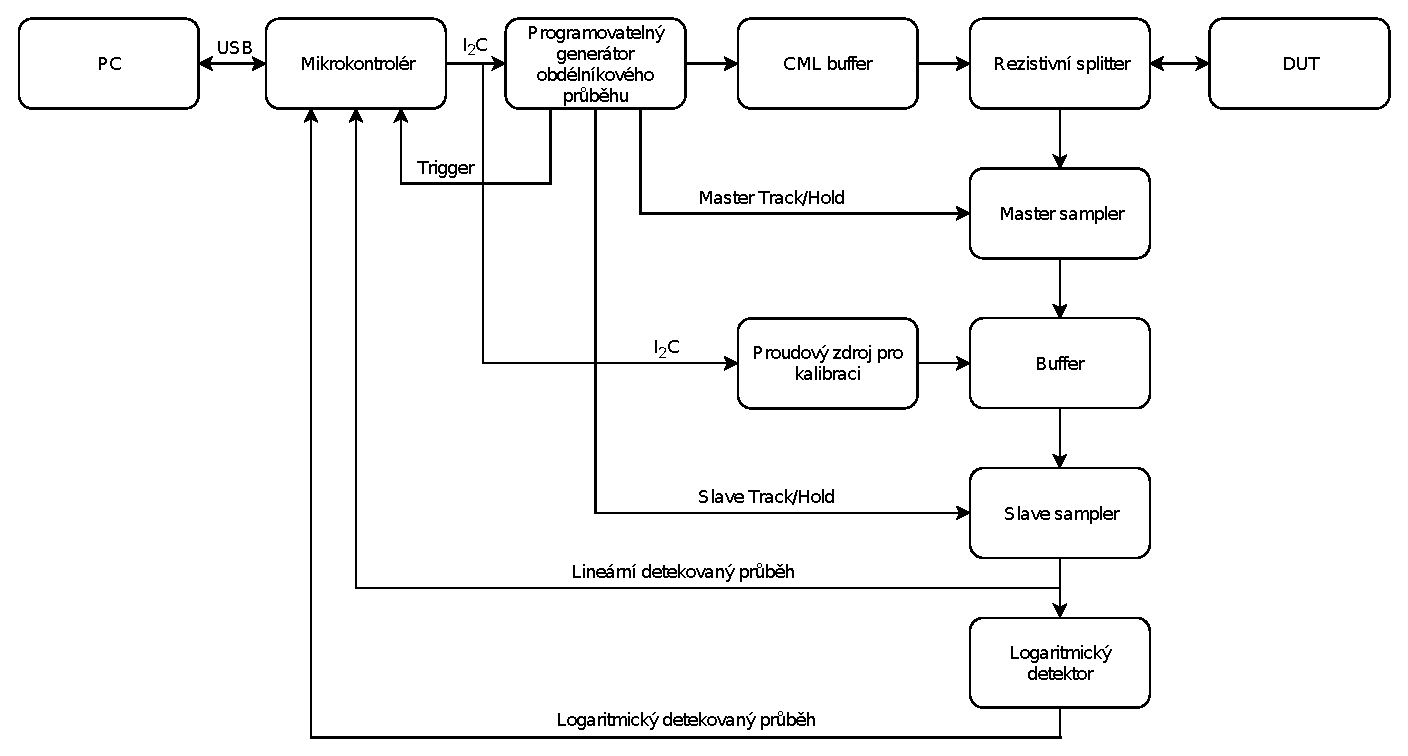
\includegraphics[width=\textwidth,keepaspectratio]{images/block_diagram.eps}\caption{Blokové zapojení reflektometru.} \label{block_diagram}
\end{figure}

Podrobnější blokové zapojení reflektometru je znázorněno na obrázku \ref{block_diagram}. V dalších částech této kapitoly jsou jenotlivé bloky popsány do hloubky.

\section{Generování potřebných hodinových signálů}
Hlavním prvkem celého zapojení je vícekanálový digitální fázový závěs, který je postaven na obvodu Si5351C-B \cite{Si5351datasheet}. Tento obvod obsahuje krystalový oscilátor, na nějž jsou zavěšeny dva interní oscilátory \acrshort{VCO}. Vnitřní blokové schéma je možné vidět na obrázku \ref{si5351_internal_architecture_overview}.

\begin{figure}[htbp]
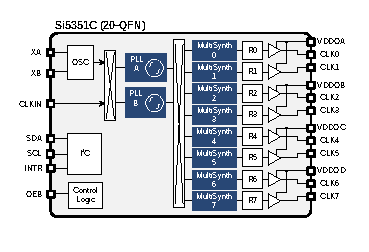
\includegraphics[width=\textwidth,keepaspectratio]{images/si5351_internal_architecture_overview.eps}\caption{Vnitřní blokové zapojení obvodu Si5351, převzato z \cite{Si5351datasheet}.} \label{si5351_internal_architecture_overview}
\end{figure}

Frekvenci těchto oscilátorů je možné nezávisle nastavit. Jejich frekvence $f_\mathrm{VCO}$ může být neceločíselným násobkem frekvence krystalového oscilátoru $f_\mathrm{XTAL}$.
\begin{equation}
f_\mathrm{VCO}=f_\mathrm{XTAL} \left(a+\dfrac{b}{c} \right)
\end{equation}
Koeficient $a$ může nabývat hodnot $\langle 15, 90 \rangle$. V neceločíselném režimu může koeficient $c$ nabývat hodnot $\langle 0, 1048575 \rangle$, koeficient $b$ pak $\langle 0, c \rangle$.
Je tedy možné nastavit frekvenci oscilátorů tak, že se liší o méně než 1 ppm. Při použití těchto dvou frekvencí jako časovacích signálů pro buzení a vzorkování je tedy možné odebírat až 1048576 vzorků. Dochází totiž k tomu, že s každou periodou se postupně hrany těchto obdélníkových signálů vůči sobě časově posunou o fixní časový krok. Tento krok je možné spočítat z nastavených frekvencí oscilátorů.

\begin{equation}
\begin{gathered}
f_\mathrm{VCO1}=f_\mathrm{XTAL} \left(a_1+\dfrac{b_1}{c_1} \right) \\
f_\mathrm{VCO2}=f_\mathrm{XTAL} \left(a_2+\dfrac{b_2}{c_2} \right)
\end{gathered}
\end{equation}

Za těmito oscilátory ještě následují děličky. Ty také umožňují neceločíselné dělení, které je ovšem nevýhodné, protože může zvyšovat fázové chvění výstupního signálu. Proto jsou použity pouze v celočíselném režimu. Děličky jsou použity kvůli omezenému vzorkovacímu kmitočtu použitého \acrshort{ADC}. Výsledkem jsou tedy dvě frekvence $f_\mathrm{OUT1}$ a $f_\mathrm{OUT2}$. Označíme-li společný dělicí poměr $d$ a za předpokladu, že $a_1=a_2=a$, $c_1=c_2=c$ a $b_2=0$:

\begin{equation}
\begin{gathered}
f_\mathrm{OUT1}=\dfrac{f_\mathrm{VCO1}}{d}=f_\mathrm{XTAL} \left(\dfrac{a+\dfrac{b_1}{c} }{d}\right) \\
f_\mathrm{OUT2}=\dfrac{f_\mathrm{VCO2}}{d}=f_\mathrm{XTAL} \left(\dfrac{a}{d}\right)
\end{gathered}
\end{equation}

Pak se během jedné periody oscilátory vůči sobě posunou o čas $T_{SHIFT}$:

\begin{equation}
\begin{gathered}
T_\mathrm{SHIFT}=T_\mathrm{OUT2}-T_\mathrm{OUT1}=\dfrac{1}{f_\mathrm{OUT2}} - \dfrac{1}{f_\mathrm{OUT1}} \\
T_\mathrm{SHIFT}=\dfrac{d}{f_\mathrm{XTAL}} \left(\dfrac{1}{a} - \dfrac{1}{a+\dfrac{b_1}{c}}\right) = \dfrac{d}{a f_\mathrm{XTAL}} \left(\dfrac{1}{1+a\dfrac{c}{b_1}}\right)
\end{gathered}
\label{equation_tshift}
\end{equation}

Pro minimalizaci fázového chvění je podle \cite{Si5351datasheet} a \cite{Si5351applicationnote} vhodné preferovat celočíselné násobení i dělení, je-li to možné. Dále může fázové chvění zmenšit i použití sudých násobitelů a dělitelů. V navrženém zapojení je tedy fázový závěs nastaven takto:

\begin{equation}
\begin{gathered}
f_\mathrm{XTAL}=\SI{25}{MHz} \\
a=24 \;\;\; b_1=24/8=3 \\
c=500000/8=62500 \;\;\; d=128 \cdot 46=5888 \\
f_\mathrm{OUT1} \doteq \SI{101902}{kHz} \doteq f_\mathrm{OUT2} \\
T_\mathrm{SHIFT} = \dfrac{46 \cdot 128}{24 \cdot 25000000} \left(\dfrac{1}{1+24 \cdot \dfrac{500000}{24}}\right) \doteq \SI{19.627}{ps}
\end{gathered}
\end{equation}

Podobný princip měření pomocí dvou oscilátorů o podobné frekvenci se již v literatuře objevil, avšak zatím nebyl implementován přímo pomocí fázového závěsu. V \cite{vernierreflectometer} byly použity dva nezávislé oscilátory. Toto řešení je sice jednodušší, avšak není možné zajistit, jak velký bude časový krok měření. Vzhledem ke skutečnosti, že oscilátory jsou závislé na teplotě a dalších vnějších vlivech, není možné zajistit ani dlouhodobou stabilitu. Při použití dvojitého fázového závěsu s neceločíselným násobitelem však je možné tuto dlouhodobou stabilitu zajistit. Krok měření je pak závislý pouze na frekvenci jediného krystalového oscilátoru. Při použití \acrshort{TCXO} může být tato stabilita velmi dobrá, na úrovni jednotek \si{ppm}.

Další podobný způsob časování vzorkování je použit v \cite{ddsfpgareflectometer}, kde je využito \acrshort{FPGA} jako \acrshort{DDS}. Výstup z této \acrshort{DDS} je filtrován dolní propustí a následně zaveden do komparátoru, římž je získáván obdélníkový řídicí signál. Řízení vzájemné polohy budicího pulzu a vzorkování je pak dosaženo nastavováním fáze sinusového signálu, který je generován \acrshort{DDS}. Tento systém umožňuje krok vzorkování v jednotkách pikosekund. Je tedy podobný vlastnostmi konstrukci popsané v této práci. Něvýhodou je však to, že autoři se příliš nezabývali generátorem impulzů, náběžná hrana použitého generátoru činí přibližně \SI{2}{ns}. Důvod, proč tak autoři učinili, je možná omezení vyplývající ze zvoleného způsobu vzorkování pomocí komparátoru a digitálního integrátoru.

\begin{figure}[htbp]
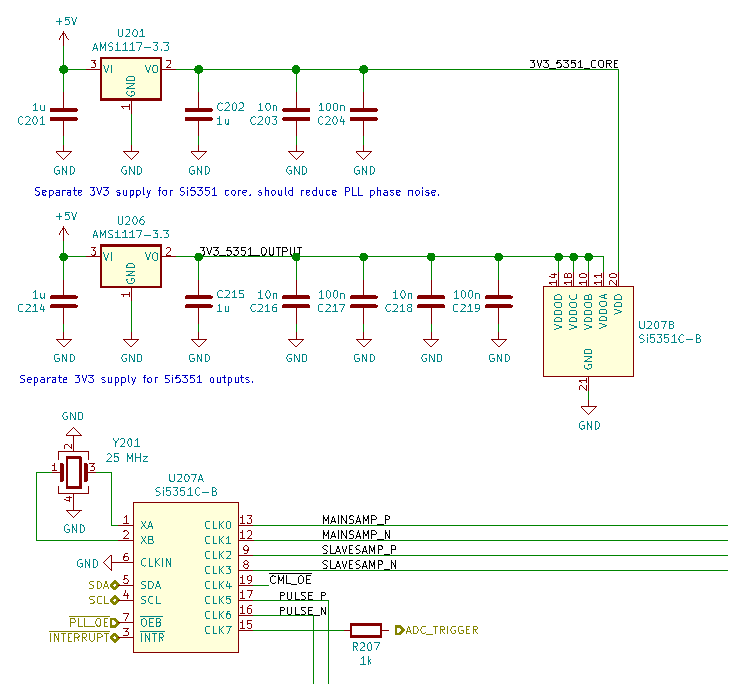
\includegraphics[width=\textwidth,keepaspectratio]{images/timing_section.eps}\caption{Zapojení hodinového generátoru Si5351.}\label{timing_section_schematic}
\end{figure}	

Zapojení hodinového generátoru s fázovým závěsem Si5351 je zobrazeno na \ref{timing_section_schematic}. Symbol obvodu je rozdělený na dvě části, U207A a U207B. Kromě samotného obvodu Si5351 je potřeba pouze referenční krystal a napájecí obvody. Napájení je rozděleno na dvě domény. První je jádro fázového závěsu, které napájí interní logické obvody a \acrshort{VCO}. Druhá napájí výstupní budiče. Toto rozdělení by mělo omezit fázový šum generovaných hodinových signálů způsobený rušením na napájení \acrshort{VCO} \cite{Si5351applicationnote}. Pro krystalový oscilátor není potřeba používat zatěžovací kondenzátory, jsou obsaženy uvnitř obvodu Si5351, je možné je nastavit v rozsahu \SIrange{4}{10}{\pico\farad}.

Výstupní budiče obvodu Si5351 jsou slučitelné jak s \acrshort{CMOS} obvody a jejich modernějšími variantami, tak i s obvody rodin \acrshort{TTL}, \acrshort{ECL}, \acrshort{CML}, \acrshort{LVDS} a podobnými. Budiče jsou proudové, proud je možné nastavit ve čtyřech krocích v rozsahu \SIrange{2}{8}{\milli\ampere} \cite{Si5351datasheet}. Tohoto faktu je využito v zapojení, 4 výstupy jsou použity přímo pro proudové buzení vzorkovacích můstků, 2 výstupy pro buzení \acrshort{CML} bufferu, jeden výstup pro synchronizaci vzorkování použitého mikrokontroléru a jeden výstup pro řízení stavu \acrshort{CML} bufferu.

Dle katalogových údajů by tento fázový závěs měl typicky dosahovat mezivrcholového fázového šumu \SI{70}{\pico\second}, maximálně  \SI{155}{\pico\second}. Dle výrobce by mělo jít o parametry v \quotedblbase nejhorším možném případě v reálné aplikaci \ldots{} skutečné vlastnosti mohou být výrazně lepší\textquotedblleft{} \cite{Si5351datasheet}. Bohužel není uvedeno, jak se tento parametr mění v závislosti na nastavení násobicích a dělicích sekcí. Není uveden ani histogram šumu, jeho frekvenční spektrum, ani efektivní hodnota. Spektrum fázového šumu je možné najít v \cite{Si5351_phase_noise_measurement}, bohužel se nejedná o ověřený zdroj.

\section{Tvorba budicího pulzu}
Pro tvorbu budicích pulzů byl vybrán obvod SY54020, který je původně určen jako \acrshort{CML} buffer. Logické obvody \acrshort{CML} používají logické úrovně referencované vůči kladnému pólu napájení, výstupy i vstupy těchto obvodů jsou přizpůsobené impedanci \SI{50}{\ohm}. Podle katalogových údajů \cite{SY54020datasheet} by měla výstupní impedance ležet v rozsahu \SIrange{45}{55}{\ohm}. Hlavní důvod pro použití tohoto bufferu je vysoká rychlost, dle katalogových údajů by měla délka náběžných a sestupných hran spadat do rozsahu \SIrange{35}{100}{\pico\second}, typicky \SI{60}{ps}. Tento údaj je udáván pro body, kde prochází náběžná hrana \SI{20}{\%} a \SI{80}{\%} mezi původním a konečným napětím. U obvodu Si5351 by podle katalogových údajů měl tento parametr být typicky \SI{1}{\nano\second}, maximálně \SI{1.5}{\nano\second}. Použitím obvodu SY54020 by tedy mělo být možné zkrátit náběžné hrany o \SIrange{90}{98}{\%} oproti přímému použití výstupu z obvodu Si5351 jako zdroje budicích pulzů. Dle katalogových údajů by špičkový aditivný fázové chvění mělo být přibližně \SI{1}{\pico\second}, tedy přibližně o dva řády lepší, než fázové chvění obvodu Si5351. Použití budiče SY54020 by tedy mělo mít zcela minimální vliv na celkovou úroveň fázového chvění.

\begin{figure}[htbp]
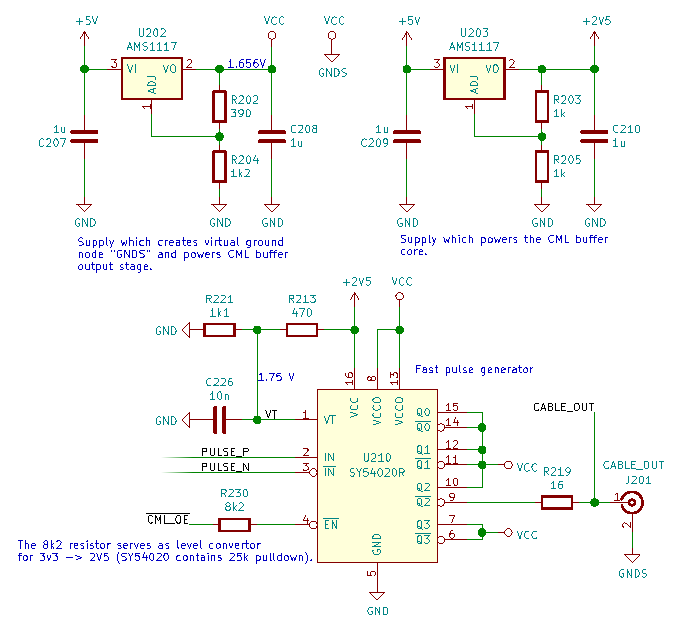
\includegraphics[width=\textwidth,keepaspectratio]{images/pulse_generator_section.eps}\caption{Zapojení generátoru budicích pulzů}\label{pulse_generator_section_schematic}
\end{figure}	

Postatná výhoda obvodu SY54020 spočívá v oddělení napájecích úrovní vstupů a výstupů tohoto obvodu. V zapojení je vstupní část obvodu napájena \SI{3.3}{\volt}, výstupní část \SI{1.65}{\volt}, tedy přesně polovičním napájecím napětím. Tato napájecí hladina označená jako VCC, a zároveň jako GNDS, je použita jako virtuální analogová země. Všechny následující analogové obvody jsou vztažené k této virtuální zemi. Díky tomu je možné k buzení vzorkovacích můstků použít přímo fázový závěs Si5351, protože můstek je tak buzen symetricky. Zapojení generátoru budicích impulzů je na obrázku \ref{pulse_generator_section_schematic}.

\section{Přizpůsobovací obvody a testovací port}
Generátor budicích impulzů z předchozího bodu je nezbytné připojit k měřicímu portu. K tomuto portu však musí být zároveň připojeny vzorkovací obvody. Proto jsou nezbytné přizpůsobovací obvody, které umožňují připojit k testovacímu portu obě tyto části při dodržení vstupní impedance. Jejich zapojení je uvedeno na obrázku \ref{match_section_schematic}.

\begin{figure}[htbp]
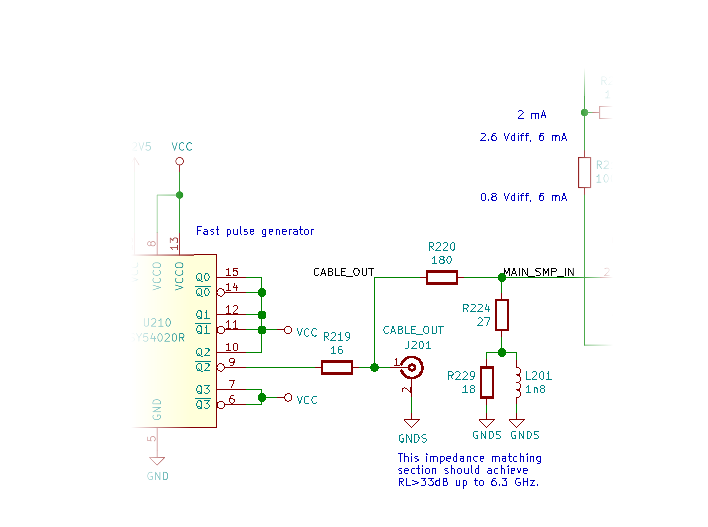
\includegraphics[width=\textwidth,keepaspectratio]{images/match_section.eps}\caption{Schéma přizpůsobovacích obvodů.}\label{match_section_schematic}
\end{figure}

Přizpůsobovací obvody jsou navrženy tak, aby bylo dosaženo co nejlepšího impedančního přizpůsobení na testovacím konektoru. Problematická je impedance vzorkovacího můstku, neboť na jeho výstupu je připojen vzorkovací kondenzátor, který způsobuje rezonanci pouzdra vzorkovacího můstku na frekvenci přibližně \SI{1.7}{\giga\hertz}. Vliv této rezonance na vstupní impedanci reflektometru je částečně potlačen použitím děliče sestaveného z odporů R220, R224 a R229 a cívky L201 (označení podle obrázku \ref{match_section_schematic}). Výsledná impedance je zakreslena v grafu \ref{input_impedance}, parametr $S_{11}$ pak v grafu \ref{input_reflection}. Simulace byla provedena bez vední T1, které se nachází na schématu \ref{ltspice_schematic}. Hodnoty použitých součástek v děliči se mezi schématy liší, protože během vývoje zařízení byly použité diodové můstky HSMS-282P vyřazeny z výroby. Jako náhrada byly vybrány diodové můstky SMS3923-081LF. Díky podrobnějšímu SPICE modelu bylo možné do simulace zahrnout i vliv parazitních vlastností pouzdra tohoto můstku, což umožnilo další optimalizace. Konečné hodnoty použitých součástek se nachází ve schématu použitém v simulaci.

\begin{figure}[htbp]
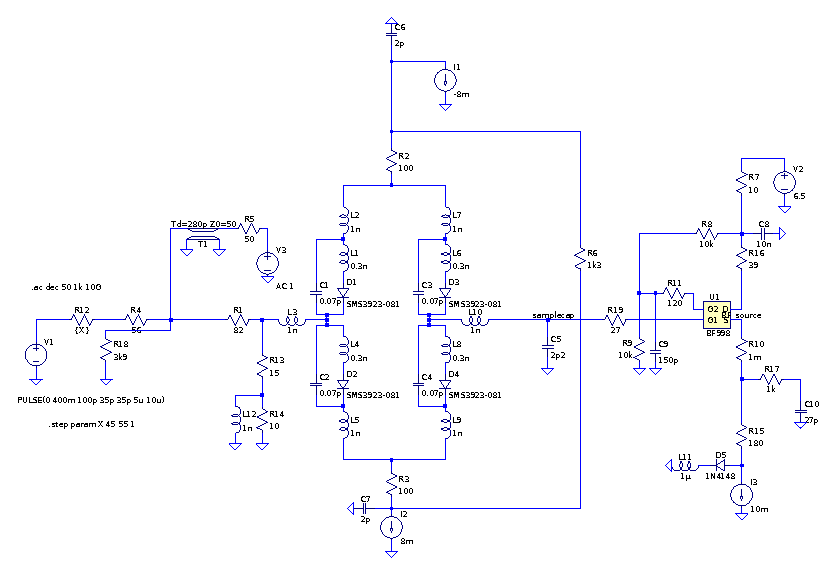
\includegraphics[width=\textwidth,keepaspectratio]{images/ltspice_schematic.eps}\caption{Schéma použité pro simulaci vstupní impedance v programu LTSpice.}\label{ltspice_schematic}
\end{figure}

\begin{figure}[htbp]
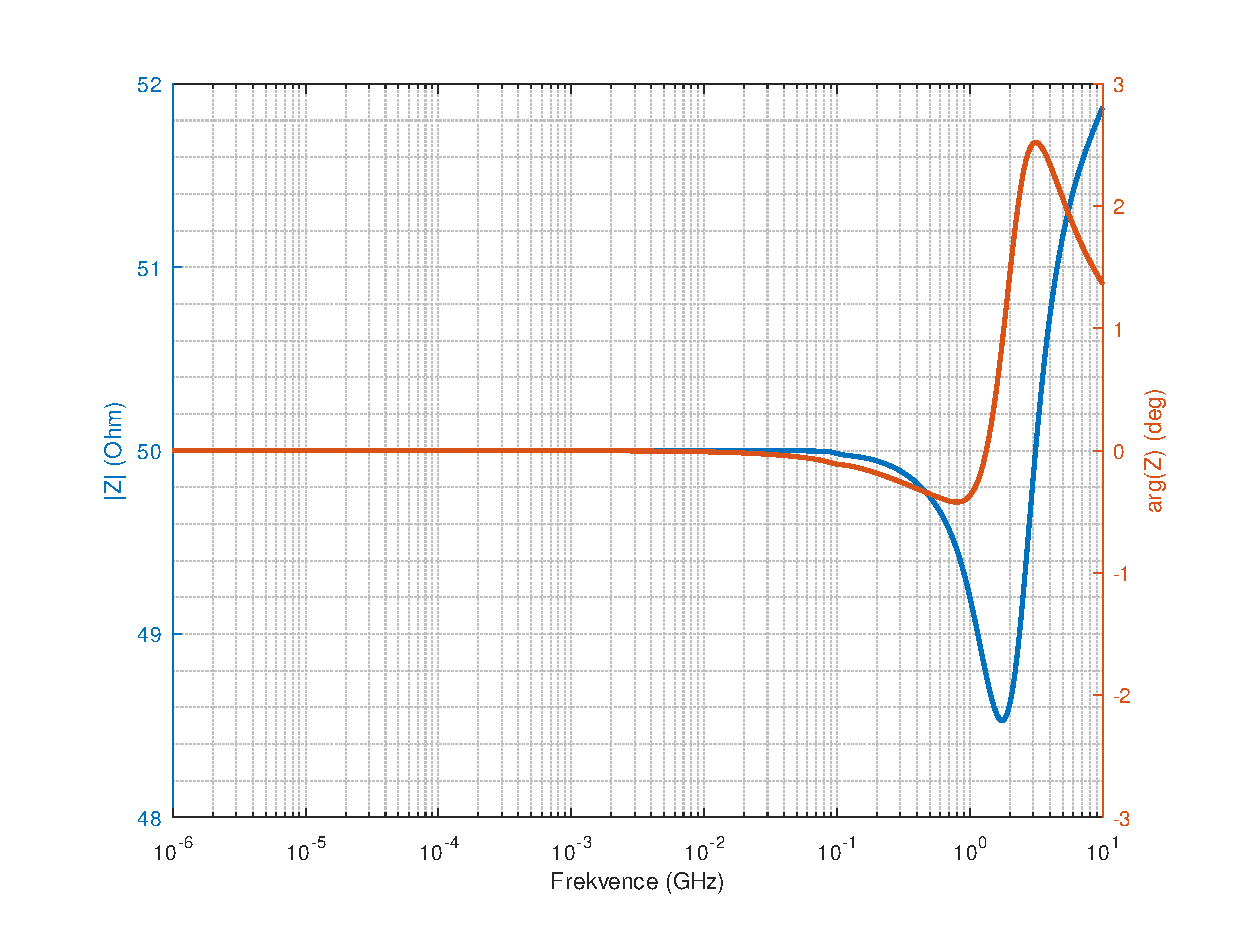
\includegraphics[width=\textwidth,keepaspectratio]{images/input_impedance.eps}\caption{Vstupní impedance reflektometru.}\label{input_impedance}
\end{figure}

\begin{figure}[htbp]
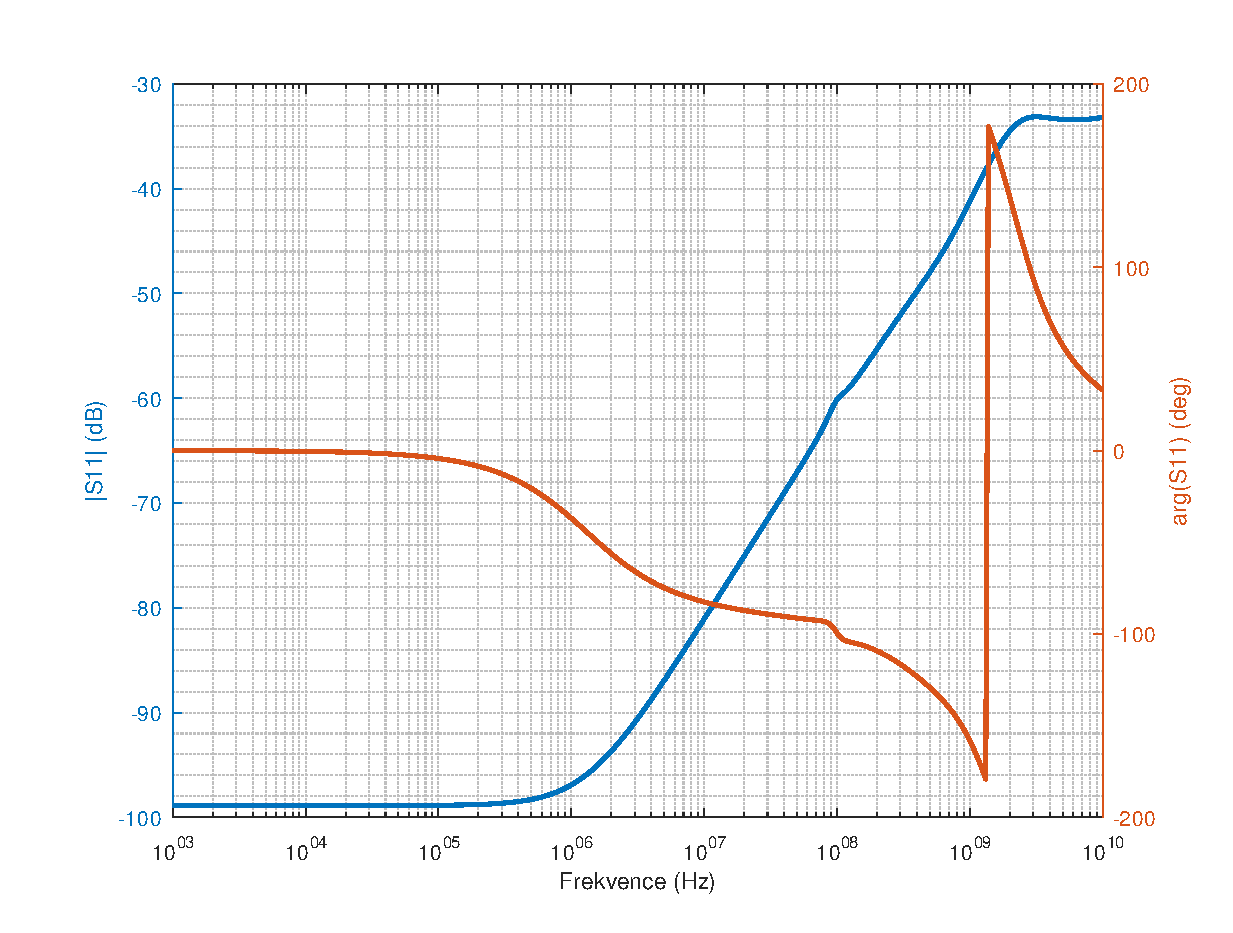
\includegraphics[width=\textwidth,keepaspectratio]{images/input_reflection.eps}\caption{Přizpůsobení vstupní impedance reflektometru.}\label{input_reflection}
\end{figure}

Vstupní impedance byla simulována do 10 GHz. V celém simulovaném pásmu se vstupní impedance odchyluje od nominálních $50~\Omega$ o méně než $\pm2~\Omega$. Parametr $\lvert S_\mathrm{11} \rvert$ je vykreslen v grafu \ref{input_reflection}. V celém rozsahu je menší než \SI{-33}{\deci\bel}, což odpovídá koeficientu odrazu $\Gamma <= 0.023$. Navržené přizpůsobení by tedy mělo být velmi dobré. Vzhledem k tomu, že konektory obvykle způsobují odraz větší, než je odraz vycházející ze simulace, měl by být klíčovým prvkem pro dosažení malého odrazu na testovacím portu kvalitní konektor a připojovací vedení. Při uvažování tolerance impedance budiče SY54020, která se pohybuje v rozsahu \SIrange{45}{55}{\ohm}, se přizpůsobení zhorší, nicméně v celém rozsahu je lepší než \SI{-30}{\deci\bel}.

\section{Vzorkovací obvody a oddělovací zesilovač}
Vzorkování je v reflektometru prováděno ve třech stupních. První stupeň je tvořený diodovým můstkem U208 (na obrázku \ref{sampler_section_schematic}) a kondenzátorem C230. Druhý stupeň vzorkování je tvořen diodovým můstkem U209 a kondenzátorem C233. Třetí stupeň probíhá uvnitř mikrokontroléru v \acrshort{ADC}.

První vzorkovací stupeň je připojen k obvodu Si5351, který proudově napájí vzorkovací můstek. Proud nastavený na budičích tohoto obvodu je \SI{8}{\milli\ampere}. V době, kdy vzorkovač sleduje vstupní signál, jsou diody sepnuty v propustné oblasti, můstek se pak chová přibližně jako rezistor o odporu jednotek \si{\ohm} zapojený mezi vstupem a vzorkovacím kondenzátorem. V okamžiku, kdy má být odebrán vzorek měřeného napětí, se obrátí směr proudu tekoucí skrz můstek, čímž se můstek rozepne. Po rozepnutí má můstek charakter kondenzátoru o kapacitě desetin pikofaradu. Aby můstek co nejméně ovlivňoval vstupní impedanci reflektometru, je připojen přes přizpůsobovací obvody. Kondenzátor C230 musí mít co nejmenší kapacitu, aby příliš kapacitně nezatěžoval vzorkovací můstek. Při použití většího kondenzátoru klesá šířka propustného pásma vzorkovače a zvětšuje se vliv vzorkovače na vstupní impedanci reflektometru. Pro potlačení kapacitního charakteru vzorkovače je v přizpůsobovacím obvodu použita kombinace R229 a L201, které částečně na vysokých frekvencích stáčí impedanci zpět k reálným hodnotám. Při použití příliš malého kondenzátoru je problematická parazitní kapacita diodového můstku v rozepnutém stavu, měřený signál pak výrazně \quotedblbase prosakuje\textquotedblleft{} do navzorkovaného signálu i v okamžiku, kdy je diodový můstek rozepnutý.

\begin{figure}[htbp]
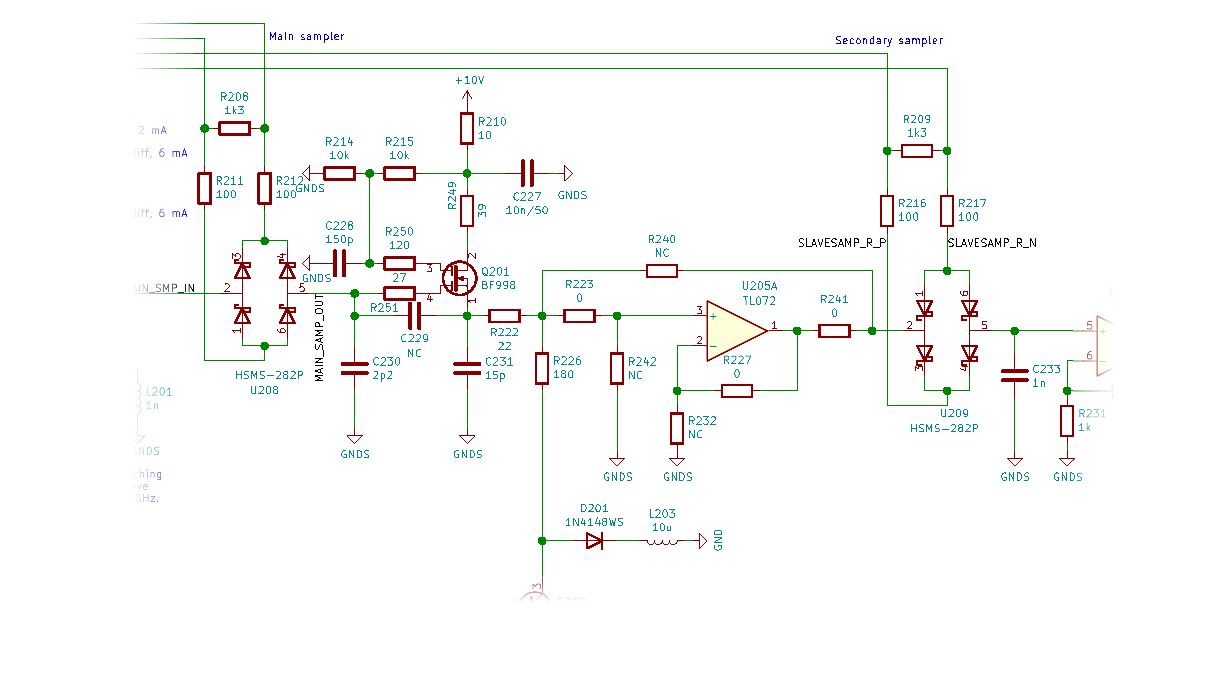
\includegraphics[width=\textwidth,keepaspectratio]{images/sampler_section.eps}\caption{Zapojení vzorkovacích obvodů.}\label{sampler_section_schematic}
\end{figure}

Vzhledem k velice malé kapacitě vzorkovacího kondenzátoru je nezbytné, aby obvody připojené k němu měly minimální vstupní proud. To by bylo možné zajistit přímo unipolárním operačním zesilovačem U205, avšak má velkou vstupní kapacitu, přibližně 27 pF \cite{oscilloscopefrontend}. Proto je použit oddělovací zesilovač s unipolárním dvouhradlovým tranzistorem BF998 s malou kapacitou hradla. Vstupní impedance oddělovacího zesilovače je přibližně do \SI{900}{\mega\hertz} takřka čistě imaginární, kapacita odpovídající této impedanci je přibližně \SI{0.6}{\pico\farad} na \SI{10}{\mega\hertz} a \SI{0.9}{\pico\farad} na \SI{1}{\giga\hertz}. Zesilovač je zapojen jako sledovač signálu s jednotkovým ziskem. V source tranzistoru je zapojen proudový zdroj kvůli minimalizaci zkreslení. Dle simulace by stejnosměrné zkreslení zesilovače mělo být lepší než \SI{0.0005}{\%}, absolutní chyba výstupního napětí je uvedena v grafu \ref{buffer_voltage_error}. Rozkmit měřeného napětí je podle simulací \SI{20}{\milli\volt}.

Při návrhu zapojení byly uvažovány i varianty s jinými tranzistory. Bohužel nebyl nalezen žádný tranzistor, který by byl  schopen pracovat do vyšších frekvencí a přitom měl nízký vstupní proudl hradla. Moderní tranzistory HEMT bohužel zpravidla mají vstupní proud v řádu mikroampérů. Rychlejší tranzistory typů MOSFET nebo MESFET se vyrábí pouze pro výkonové aplikace. Ke vhodným tranzistorům typu JFET se bohužel dodávají pouze S-parametry a nejsou dostupné parametry pro SPICE modely. Nakonec tedy byl zvolen tranzistor BF998. 

Maximální hodnotu kapacity kondenzátoru C230 určuje i oddělovací zesilovač. Při kapacitě větší než \SI{1.5}{\pico\farad} se oddělovací zesilovač rozkmital, což bylo zjištěno v zapojení během testování. Následně byla tato skutečnost potvrzena simulací a opravena. Proto jsou v zesilovači použity odpory R249, R250 a R251. R251 omezuje kladnou zpětnou vazbu a tlumí rezonanci páru U208~--~C230, čímž je zabráněno rozkmitání zesilovače. Odpor R249 nadále zeslabuje tuto kladnou zpětnou vazbu. Odpor R250 zvětšuje vstupní impedanci zesilovače a zvětšuje šířku pásma tohoto oddělovacího stupně. Kondenzátor C231 není v konečném zapojení použit, neboť zmenšoval použitelnou šířku pásma zesilovače a zhoršoval stabilitu zapojení. Přenosová charakteristika oddělovacího zesilovače je uvedena v grafu \ref{frequency_transfer_function_bf}.Podle těchto odsimulovaných výsledků by měla být 6\si{\deci\bel} šířka pásma přibližně \SI{5.9}{\giga\hertz}.

\begin{figure}[htbp]
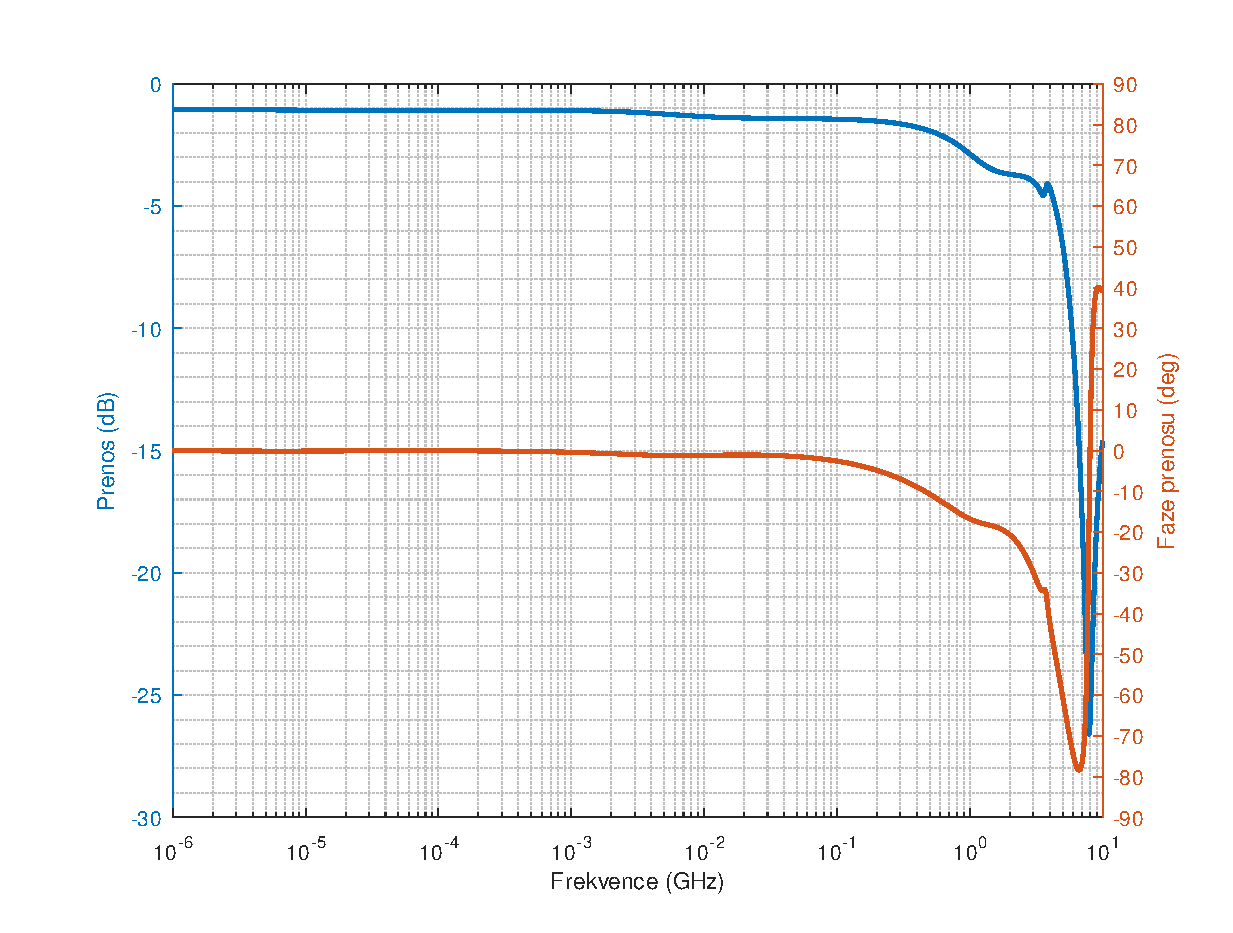
\includegraphics[width=\textwidth,keepaspectratio]{images/frequency_transfer_function_BF.eps}\caption{Přenos oddělovacího zesilovače.}\label{frequency_transfer_function_bf}
\end{figure}

Celková přenosová charakteristika od testovacího portu až k výstupu oddělovacího zesilovače je uvedena v grafu \ref{frequency_transfer_function_all}. 6\si{\deci\bel} šířka pásma pak činí přibližně \SI{1.93}{\giga\hertz}.

\begin{figure}[htbp]
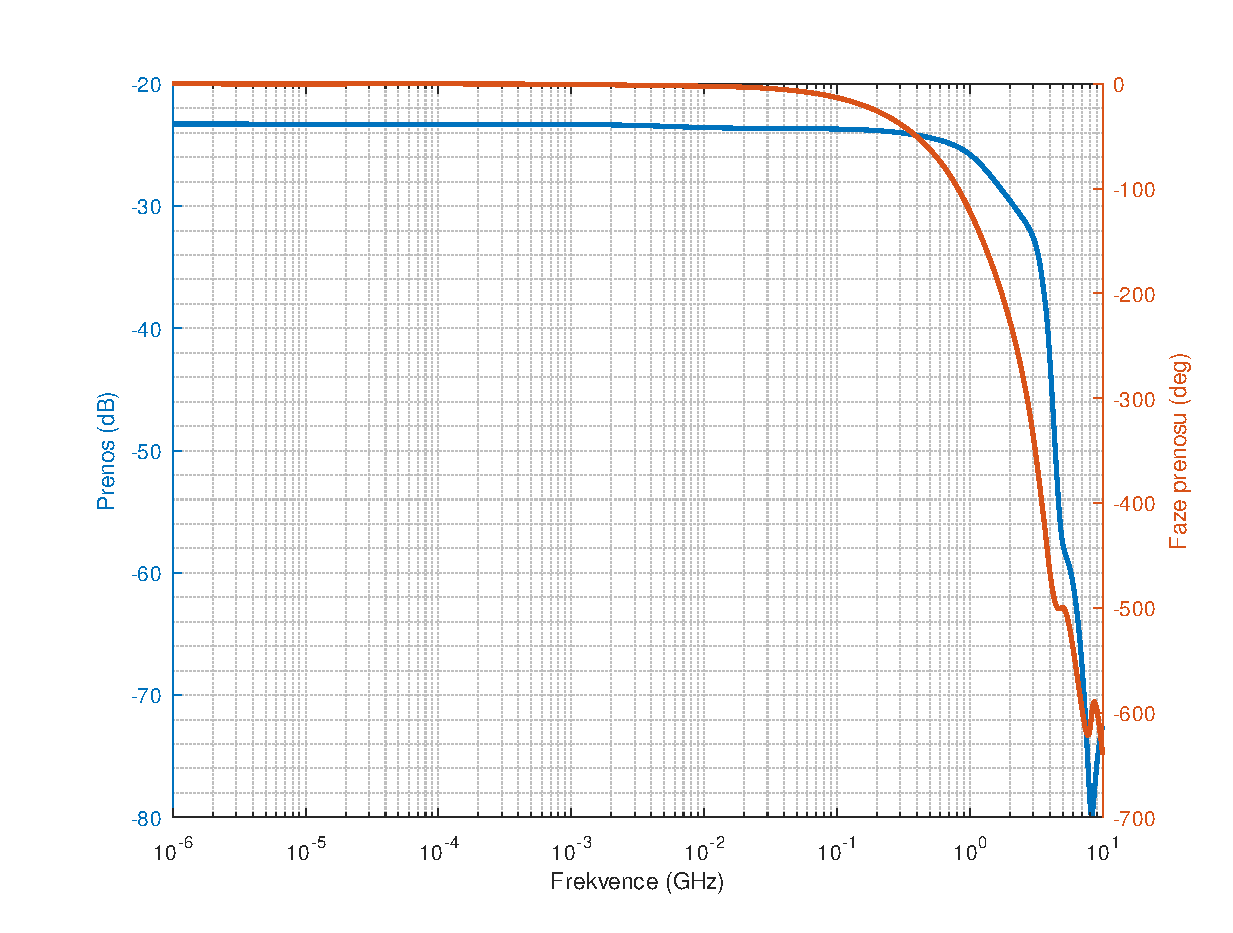
\includegraphics[width=\textwidth,keepaspectratio]{images/frequency_transfer_function_all.eps}\caption{Přenos celého systému přizpůsobení-vzorkovač-zesilovač.}\label{frequency_transfer_function_all}
\end{figure}

Simulace nebyla provedena s idealizovaným proudovým zdrojem, ale již v zapojení, které je uvedeno na schématu \ref{sampler_section_schematic}. Simulovaná data by tak měla lépe odpovídat realitě. Důvod, proč na schématu \ref{ltspice_schematic} není uvedeno celé zapojení proudového zdroje, ale jen idealizovaného zdroje, je časová náročnost výpočtů. Při simulacích vstupní impedance má tato část minimální vliv na výsledky, ale výrazně zpomaluje výpočty, proto byla ze simulací týkajících se vstupní impedance a tranzientních simulací oddělovacího zesilovače vynechána. Celé zapojení proudového zdroje je vidět na schématu \ref{current_source_section_schematic}.

\begin{figure}[htbp]
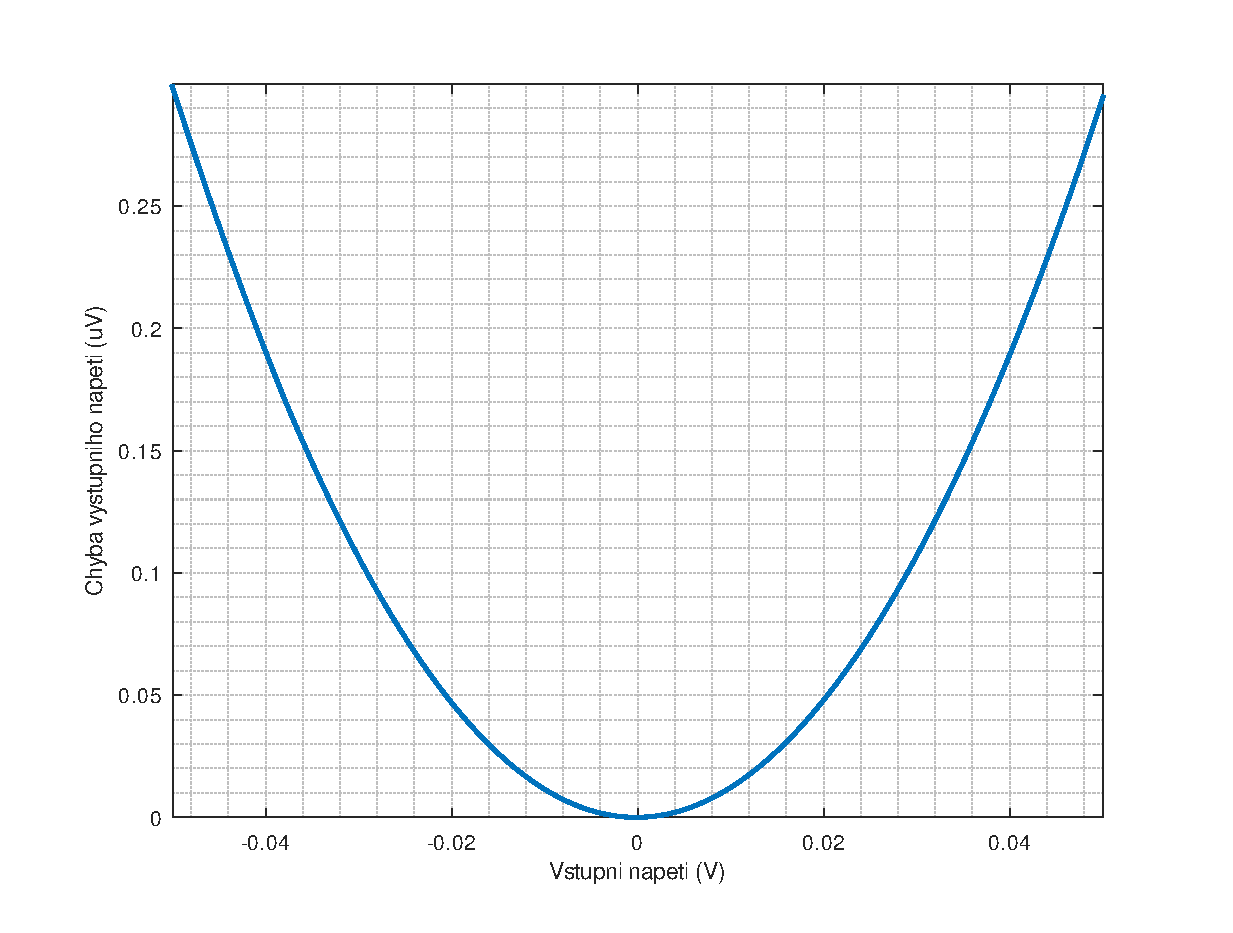
\includegraphics[width=\textwidth,keepaspectratio]{images/transfer_characteristic.eps}\caption{Absolutní chyba linearity oddělovacího zesilovače.}\label{buffer_voltage_error}
\end{figure}

\begin{figure}[htbp]
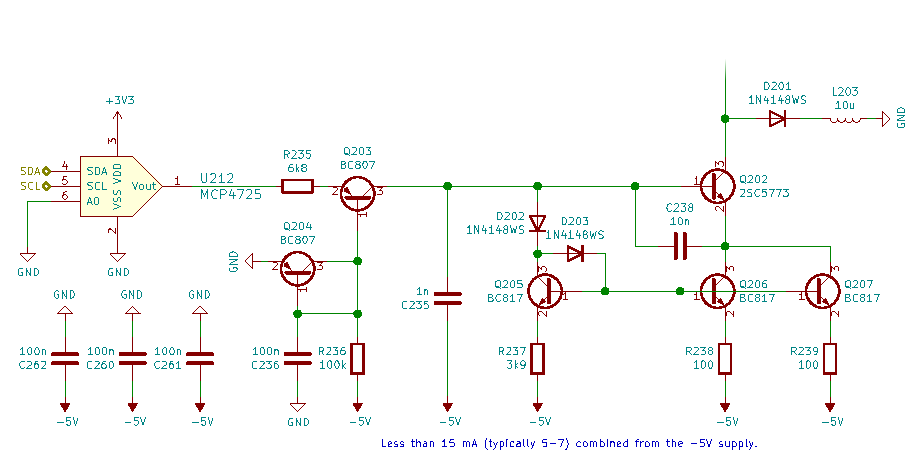
\includegraphics[width=\textwidth,keepaspectratio]{images/current_source_section.eps}\caption{Zapojení proudového zdroje.}\label{current_source_section_schematic}
\end{figure}

Proudový zdroj na schématu \ref{current_source_section_schematic} napájí oddělovací zesilovač. Zdroj je řízen \acrshort{DAC}, je možné jej nastavit v rozsahu \SIrange{0}{15.9}{\si{mA}} v 4096 krocích po přibližně \SI{3.88}{\micro\ampere}. Zroj je určen k autokalibraci reflektometru, umožňuje stejnosměrné posunutí měřeného signálu. Tento autokalibrační proces je nezbytný kvůli výrobním tolerancím a teplotní závislosti unipolárního dvouhradlového tranzistoru BF998. Proudový zdroj je zapojen jako kaskodové proudové zrcadlo. Odpor R235 spolu s tranzistory Q203 a Q204 slouží jako převodník z napětí na proud. Tranzistory Q202, Q205, Q206 a Q207 tvoří proudové zrcadlo. V emitorech tranzistorů jsou zapojeny odpory, čímž se zrcadlo podobá Widlarově proudovému zrcadlu se zesilovacím poměrem přibližně 60. Tranzistor Q202 je vysokofrekvenční typ s $f_T=\SI{6}{\giga\hertz}$ při \SI{8}{\milli\ampere} a nízkou výstupní kapacitou kolektoru, maxímálně $C_\mathrm{ob}<\SI{1.8}{\pico\farad}$. Pro ochranu tranzistoru Q202 před lavinovým průrazem během zapínání reflektometru a autokalibrace je použita dioda D201, která omezuje napětí kolektor-emitor na tranzistoru Q202 na přibližně \SI{4}{\volt}, průrazné napětí tranzistoru je dle katalogových údajů \SI{6}{\volt}. Proudový zdroj je navržen tak, že není možné nastavit proud emitorem tranzistoru Q202 větší než \SI{15}{\milli\ampere}, přičemž povolený trvalý proud je \SI{50}{\milli\ampere}. Tranzistor by tedy měl být kompletně ochráněn před poškozením. Pro potlačení vlivu kapacity diody D201 na přenos oddělovacího zesilovače na vysokých frekvencích je použita cívka L203.

\begin{figure}[htbp]
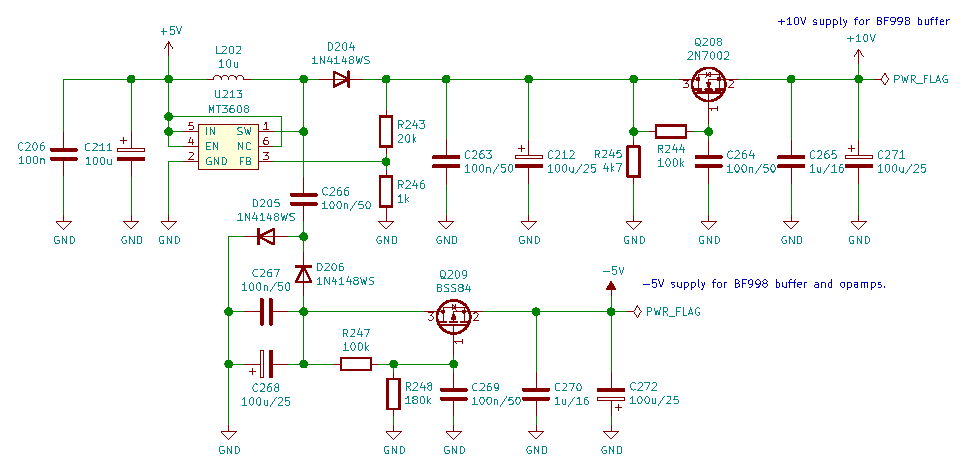
\includegraphics[width=\textwidth,keepaspectratio]{images/power_supply_section.eps}\caption{Zapojení napájecích zdrojů vzorkovacích obvodů.}\label{analog_source_section_schematic}
\end{figure}

Napájecí zdroj operačních zesilovačů, proudového zdroje a oddělovacího zesilovače je na schématu \ref{analog_source_section_schematic}. Zdroj je napájen z \SI{5}{\volt} získávaných z USB. Jádrem je spínaný zdroj MT3608 pracující na frekvenci \SI{2}{\mega\hertz}, který je nastaven na napětí \SI{12.6}{\volt}. Tato napájecí větev je filtrována aktivním filtrem s tranzistorem Q208. Napájecí hladina \SI{12.6}{\volt} je filtrována RC článkem R244-C264. Toto vyfiltrované napětí je zapojeno do gate tranzistoru Q208, který je zapojen jako sledovač. Teoreticky je tak možné zajistit značné potlačení zvlnění napětí na napájecí větvi. Výsledkem je vyfiltrované nestabilizované napětí přibližně \SI{10}{\volt}. Potlačení zvlnění by dle simulace mělo být přibližně \SI{-128}{\deci\bel} na frekvenci \SI{2}{\mega\hertz}, kde pracuje spínaný zdroj. Přenosová charakteristika tohoto aktivního filtru je na grafu \ref{analog_source_filter_transfer}, je vyznačená modře.

Záporná napájecí větev je získávána z téhož zdroje pomocí nábojové pumpy tvořené kondenzátory C266 -- C268 a diodami D205 a D206. Výsledné napětí je přibližně \SI{-12}{\volt}. Tranzistor Q209 opět tvoří aktivní filtr. Odporovým děličem je nastaveno výstupní napětí přibližně \SI{-5}{\volt}. Potlačení zvlnění by dle simulace mělo být přibližně \SI{-134}{\deci\bel} na frekvenci \SI{2}{\mega\hertz}, kde pracuje spínaný zdroj. Přenosová charakteristika tohoto aktivního filtru je na grafu \ref{analog_source_filter_transfer}, je vyznačená oranžově.

Za předpokladu, že simulace odpovídají reálnému chování navržených obvodů, mělo by být zvlnění na napájecích větvích způsobené spínaným zdrojem potlačeno aktivními filtry natolik, že by nemělo být měřitelné a nemělo by nijak ovlivňovat měření.

\begin{figure}[htbp]
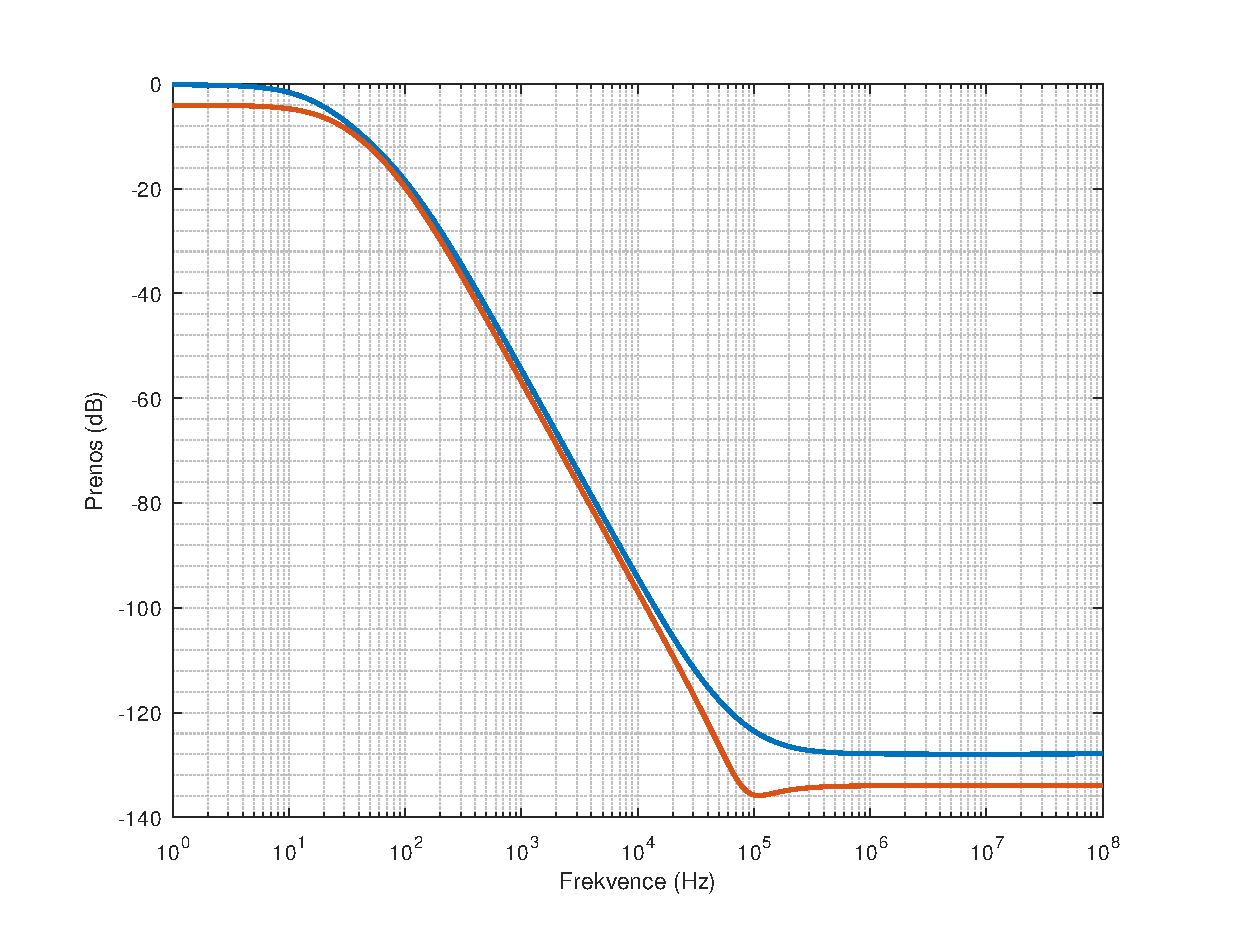
\includegraphics[width=\textwidth,keepaspectratio]{images/denoiser_transfer_function.eps}\caption{Přenosová charakteristika aktivních napájecích filtrů.}\label{analog_source_filter_transfer}
\end{figure}

Za oddělovacím zesilovačem následuje jednotkový sledovač s operačním zesilovačem TL072, který slouží ke snížení výstupní impedance oddělovacího zesilovače. Výstup tohoto zesilovače je opět vzorkován pomocí vzorkovacího můstku U209 do \SI{1}{\nano\farad} kondenzátoru. Oddělovací zesilovač má sice vysokou impedanci, takže téměř nezpůsobuje drift napětí na vzorkovacím kondenzátoru C230, nicméně vzhledem ke svodovému proudu vzorkovacího můstku U208 je tento drift nenulový. Proto těsně před sepnutím můstku U208 se rozepne můstek U209. Vzhledem k tomu, že kapacita kondenzátoru C233 je o 3 řády větší, než kapacita kondenzátoru C230, je i výsledný drift o 3 řády menší. Napětí po tomto sekundárním vzorkování je zesíleno v zesilovači U205 na schématu \ref{secondary_sampler_section_schematic}.

\section{Logaritmický detektor}

Toto navzorkované napětí je převáděno na logaritmickou podobu pomocí logaritmického detektoru AD8307. Logaritmický detektor byl použit pro rozšíření dynamického rozsahu měření dvanáctibitového \acrshort{ADC}. Bohužel, v rámci testování se ukázalo, že šum vzorkovacích obvodů je příliš velký a logaritmický detektor nepřinášel žádné zpřesnění měřených hodnot. Změřená závislost výstupního napětí logaritmického detektoru na kódovém slově \acrshort{DAC} je v grafu \ref{log_function_graph_whole}, přiblížená problematická oblast v grafu \ref{log_function_graph_zoomed}.

\begin{figure}[htbp]
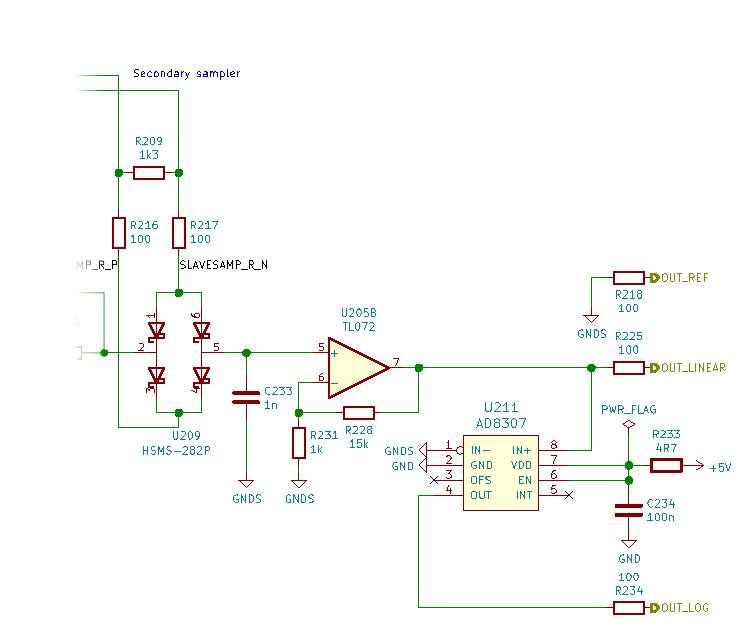
\includegraphics[width=\textwidth,keepaspectratio]{images/secondary_sampler_section.eps}\caption{Schéma sekundárního vzorkovače a logaritmického detektoru.}\label{secondary_sampler_section_schematic}
\end{figure}


\begin{figure}[htbp]
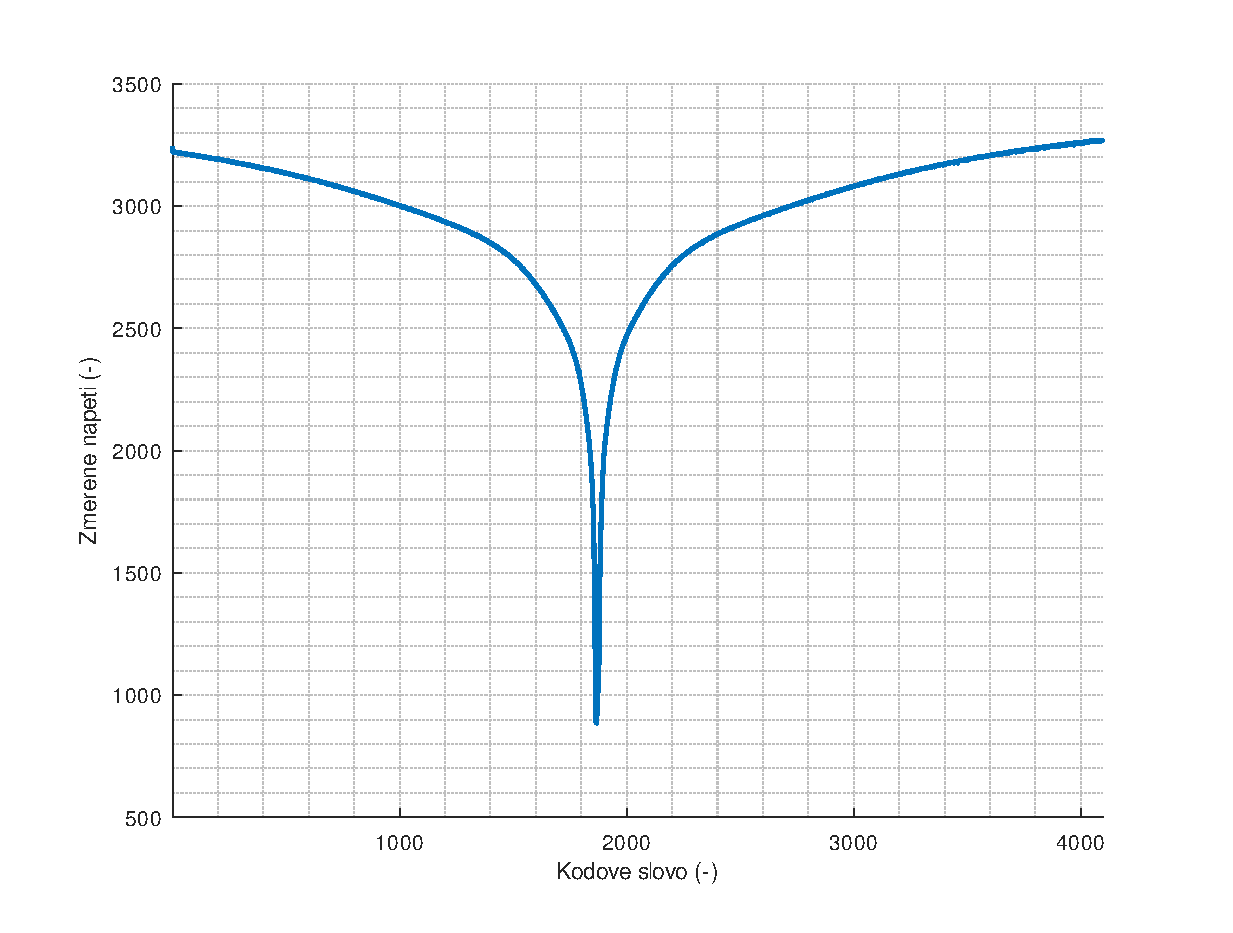
\includegraphics[width=\textwidth,keepaspectratio]{images/log_function_graph_whole.eps}\caption{Změřená závislost výstupního napětí na kódovém slově DAC, celkové zobrazení.}\label{log_function_graph_whole}
\end{figure}

\begin{figure}[htbp]
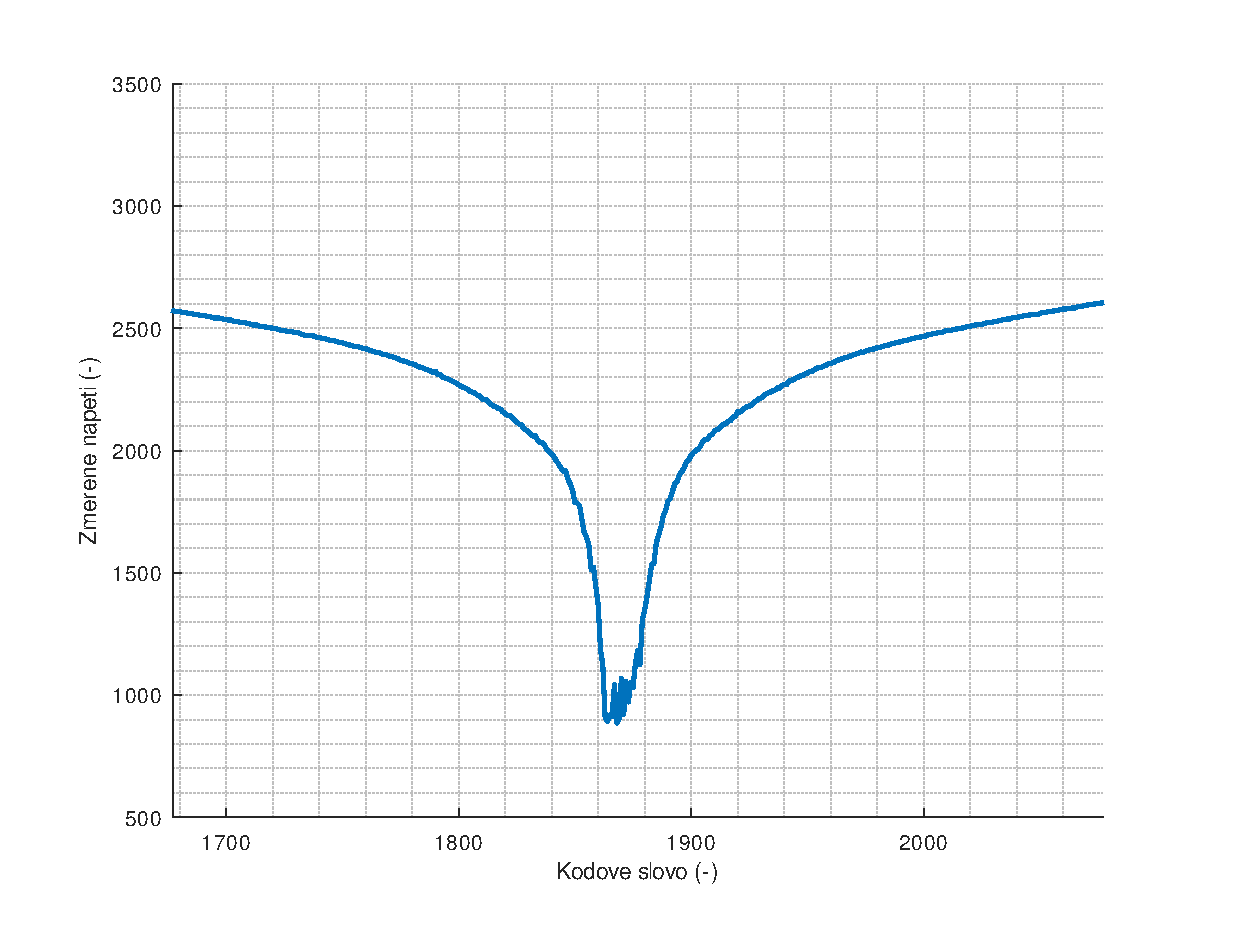
\includegraphics[width=\textwidth,keepaspectratio]{images/log_function_graph_zoomed.eps}\caption{Změřená závislost výstupního napětí na kódovém slově DAC, výřez problematické oblasti.}\label{log_function_graph_zoomed}
\end{figure}

\section{Digitalizace měřeného průběhu}
Navzorkovaný průběh je třeba pro zpracování zdigitalizovat. K tomuto účelu je použit interní \acrshort{ADC} použitého mikrokontroléru STM32F103. Tento převodník má rozlišení 12~bitů a maximální vzorkovací kmitočet \SI{1}{\megasample}. Podstatná výhoda interního převodníku je automatizace obsluhy měření. Digitalizace je synchronizována se vzorkováním, obvod Si5351 generuje synchronizační signál, kterým se digitalizace spouští. Ihned po dokončení digitalizace se vyvolává přerušení, které změřený vzorek zpracuje. Tento proces by bylo možné ještě zjednodušit použitím DMA v procesoru, avšak bylo zvoleno řešení s přerušením, protože přerušení řeší i průměrování a další úkony. Zapojení mikrokontroléru je vyobrazeno na schématu \ref{microcontroller_section}.

\begin{figure}[htbp]
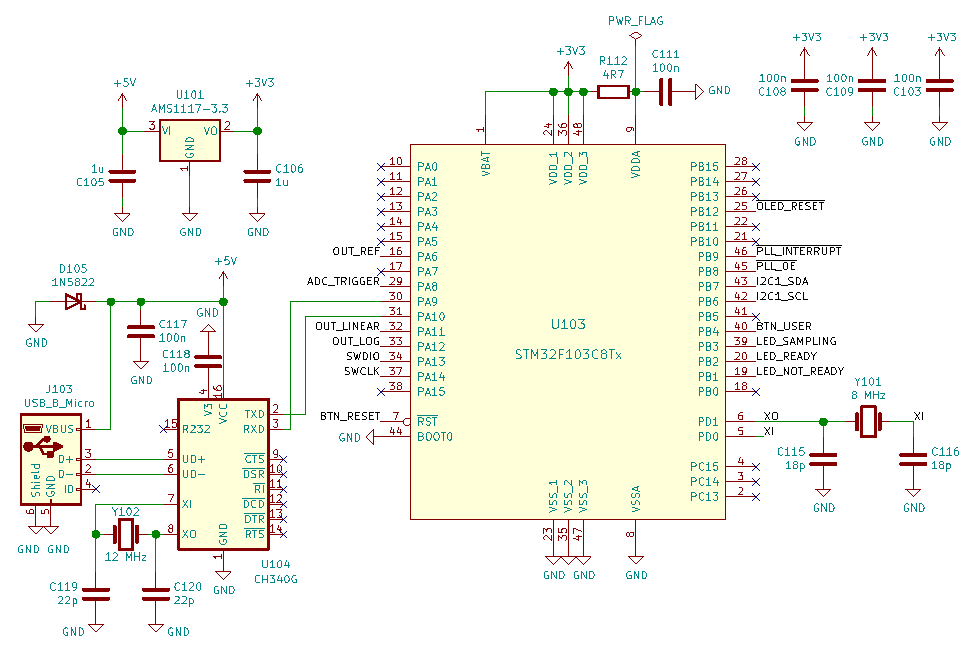
\includegraphics[width=\textwidth,keepaspectratio]{images/microcontroller_section.eps}\caption{Zapojení mikrokontroléru.}\label{microcontroller_section}
\end{figure}

\section{Komunikace s počítačem}
Komunikace reflektometru s počítačem je zajištěna pomocí virtuálního sériového portu. Ten je tvořen převodníkem CH340G, který podporuje standardní přenosové rychlosti, navíc nabízí i nestandardní rychlosti až do \SI{2}{\mega\baud}. Pro komunikaci s reflektometrem slouží ovládací software napsaný v prostředí Octave.

\section{Navržená deska plošných spojů}
Plošný spoj reflektometru byl nakreslen v návrhovém prostředí KiCAD. Vysokofrekvenční část spojů zahrnuje pouze cestu mezi konektorem, budičem a vzorkovačem. Tato cesta je dlouhá pouze několik milimetrů. Proto byl spoj navržen s předpokladem, že na takto krátkou vzdálenost není nezbytné použít materiál určený pro vysokofrekvenční zapojení. Byl proto použit obyčejný substrát typu FR-4 o tloušťce \SI{0.6}{\milli\meter}, motiv je pouze oboustranný. Tloušťka byla zvolena tak, aby koplanární vedení nemusela být širší než přibližně \SI{1}{\milli\meter} při mezeře mezi vedením a zemnicí plochou větší než \SI{0.2}{\milli\meter}. Požadavek na mezeru vychází z běžných výrobních požadavků a tolerancí výrobců plošných spojů. Navržená a vyrobená deska plošných spojů je vyfocena na obr. \ref{pcb_top_unassembled} a \ref{pcb_bottom_unassembled}. Osazená a otestovaná deska plošných spojů je na obrázcích \ref{pcb_top_assembled} a \ref{pcb_bottom_assembled}. Velké hnědé součástky, které jsou osazeny z obou stran desky plošných spojů, jsou kondenzátorová pole, která slouží ke spojení virtuální a skutečné signálové země pro vysoké frekvence, ohraničují celou oblast virtuální země. Okolí testovacího portu s koplanárním vedením je na obr. \ref{pcb_coplanar}.

\begin{figure}[htbp]
\includegraphics[width=\textwidth,height=10cm,keepaspectratio]{images/pcb/pcb_top.jpg}\caption{Vrchní strana desky plošných spojů, neosazená.}\label{pcb_top_unassembled}
\end{figure}

\begin{figure}[htbp]
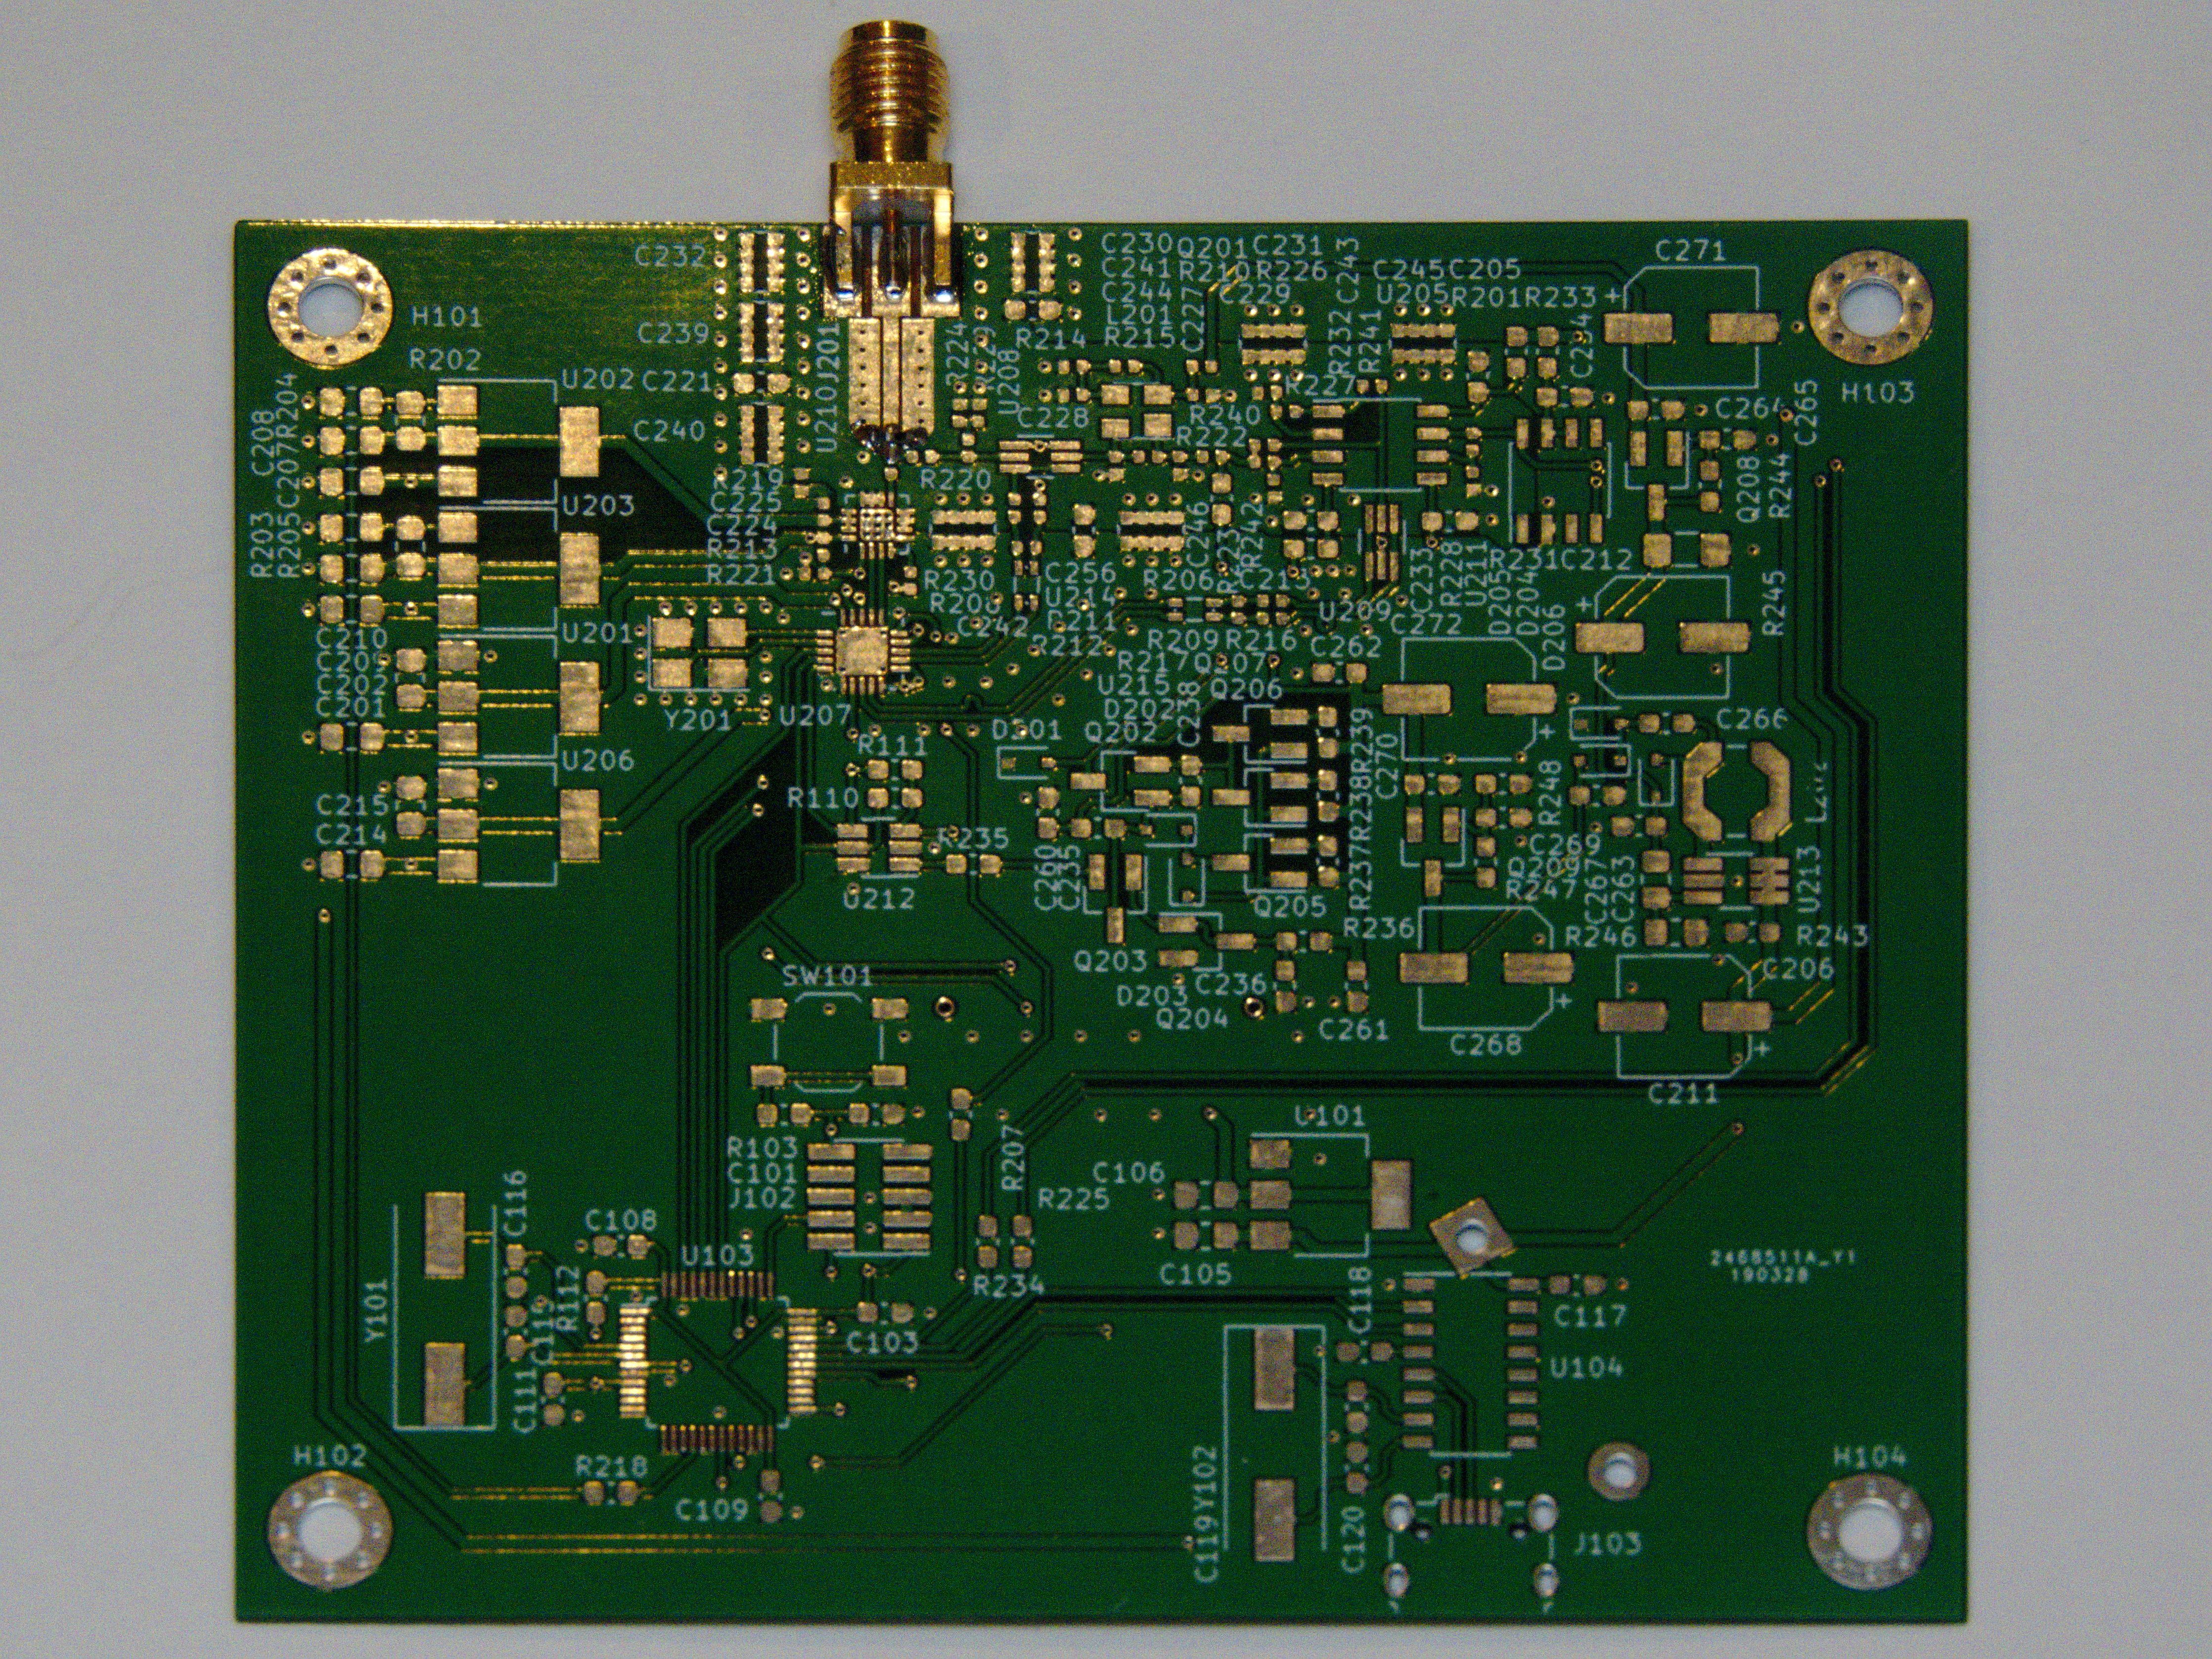
\includegraphics[width=\textwidth,height=10cm,keepaspectratio]{images/pcb/pcb_bottom.jpg}\caption{Spodní strana desky plošných spojů, neosazená.}\label{pcb_bottom_unassembled}
\end{figure}

\begin{figure}[htbp]
\includegraphics[width=\textwidth,height=10cm,keepaspectratio]{images/pcb/pcb_top_assembled.jpg}\caption{Vrchní strana desky plošných spojů, osazená.}\label{pcb_top_assembled}
\end{figure}

\begin{figure}[htbp]
\includegraphics[width=\textwidth,height=9.5cm,keepaspectratio]{images/pcb/pcb_bottom_assembled.jpg}\caption{Spodní strana desky plošných spojů, osazená.}\label{pcb_bottom_assembled}
\end{figure}

\begin{figure}[htbp]
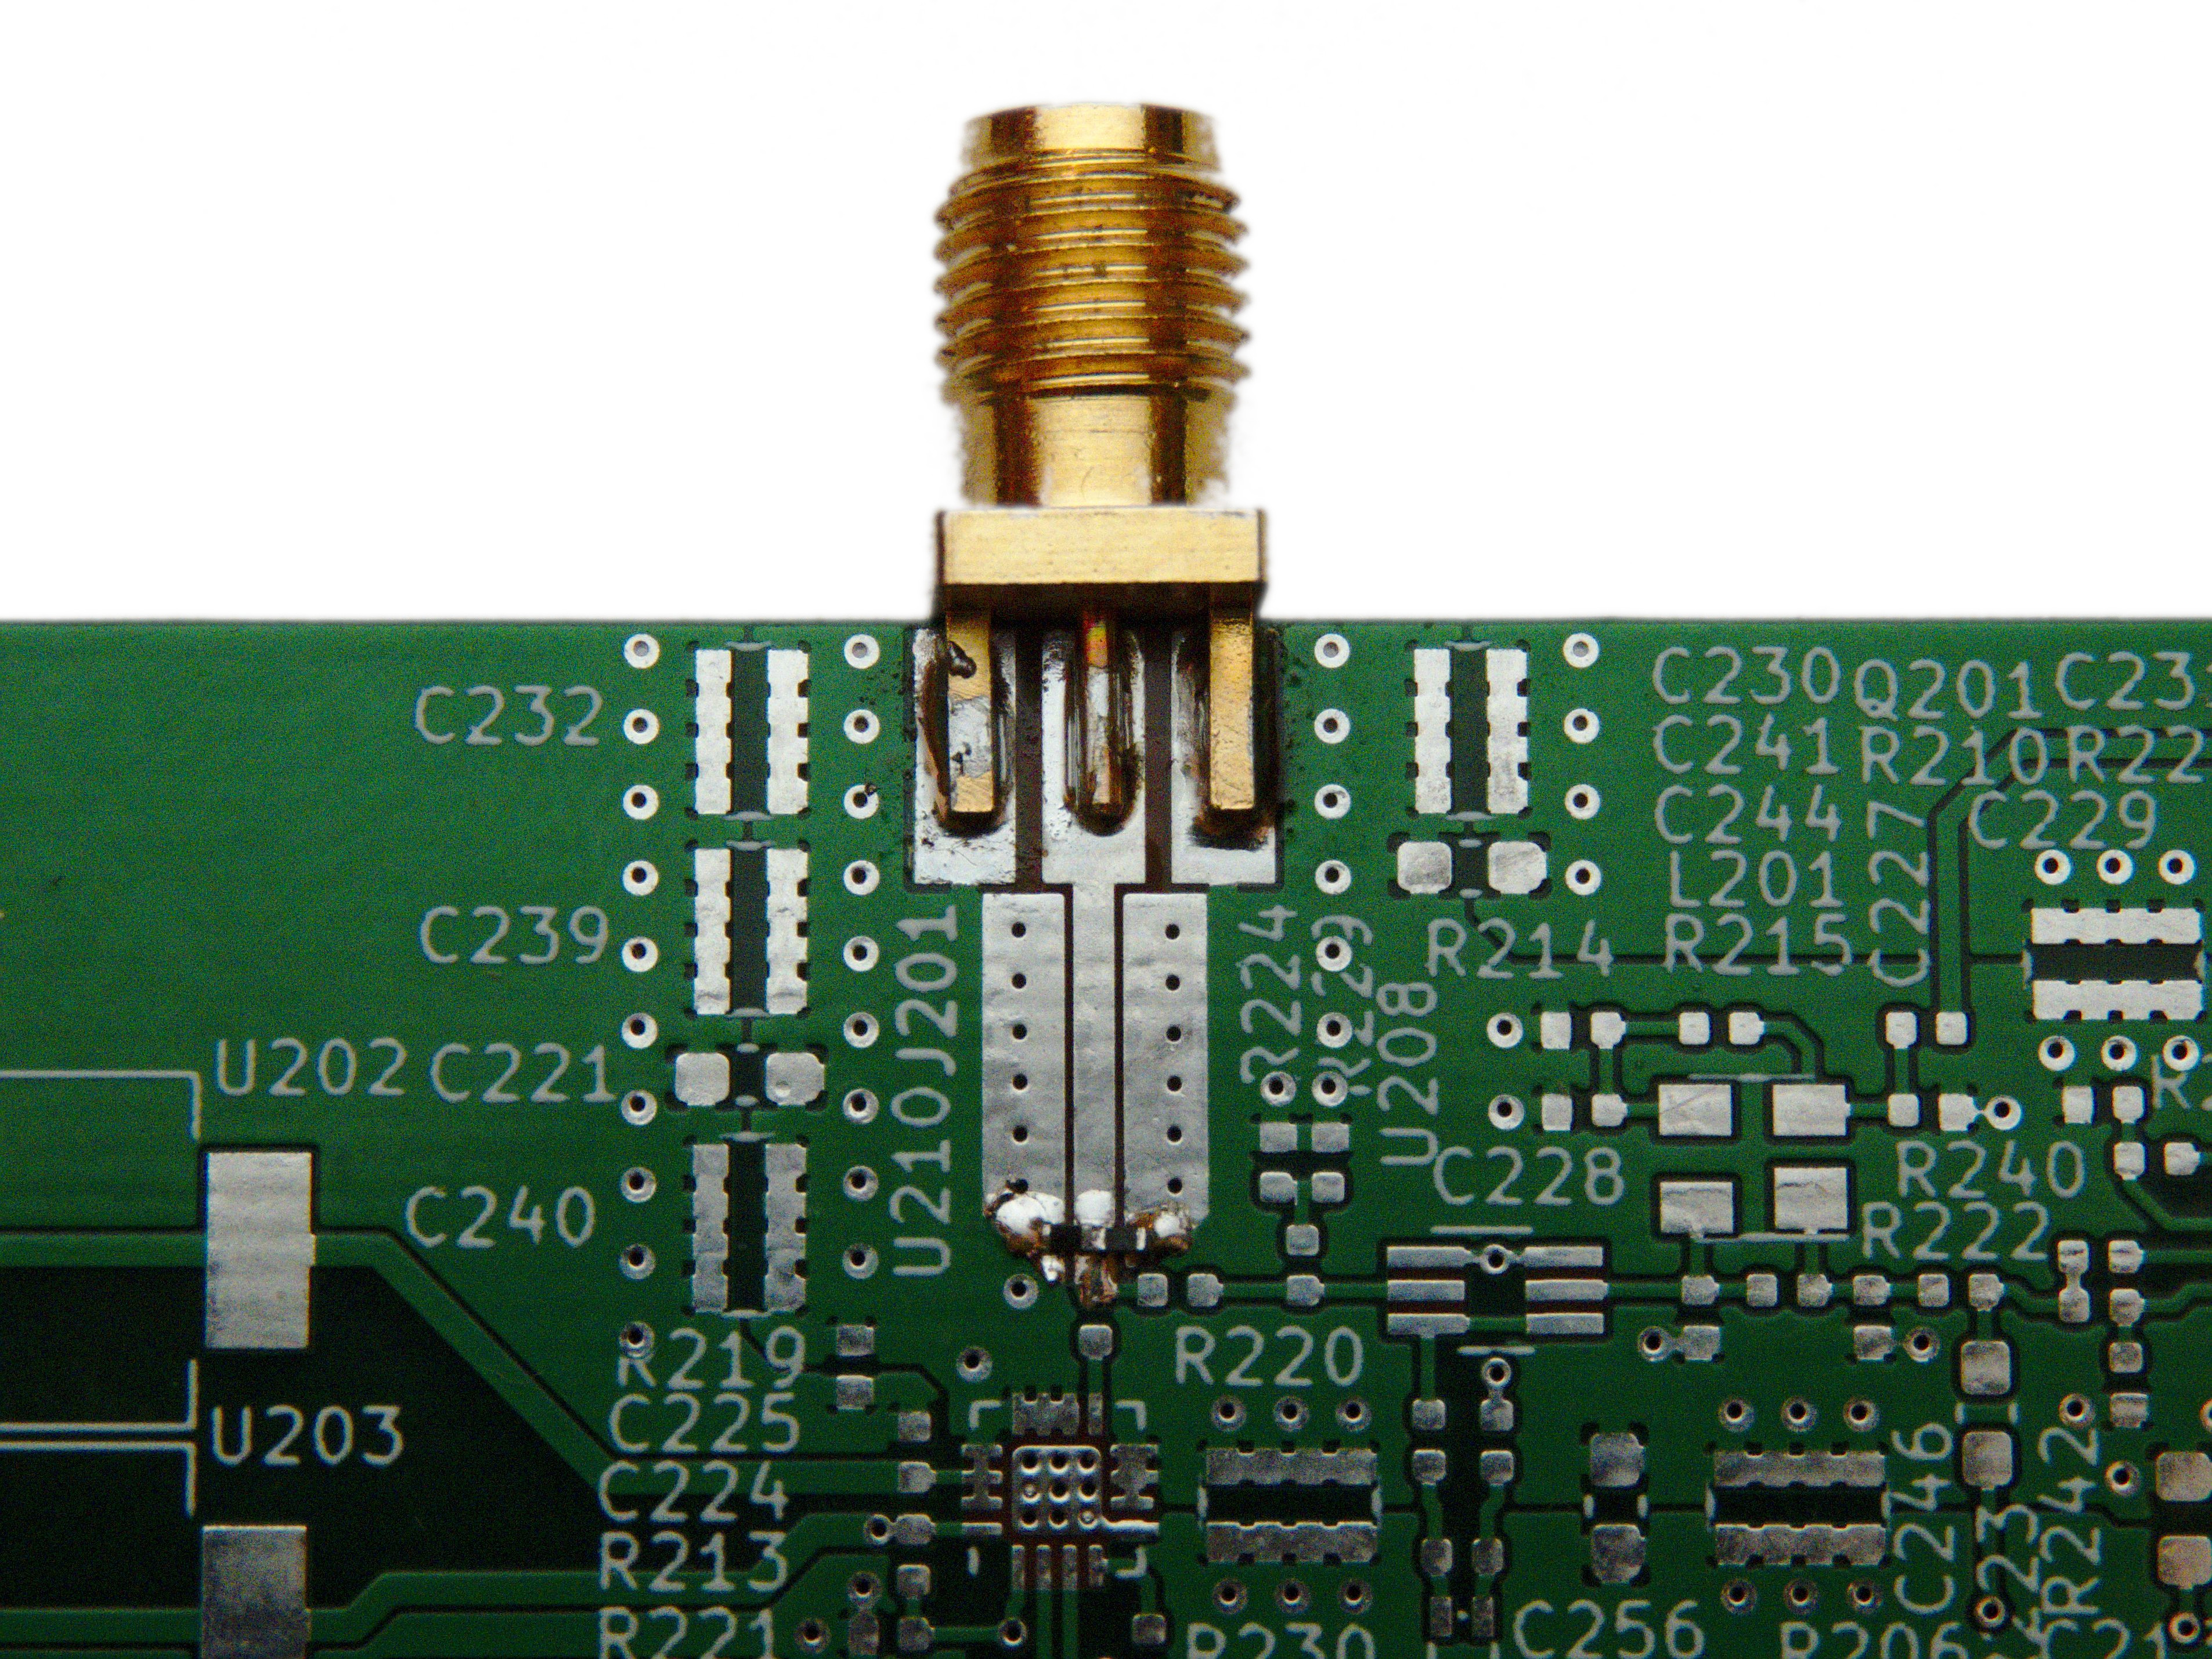
\includegraphics[width=\textwidth,height=10cm,keepaspectratio]{images/pcb/pcb_coplanar.jpg}\caption{Testovací konektor, koplanární vedení a motiv budiče a vzorkovače.}\label{pcb_coplanar}
\end{figure}

Na obr. \ref{pcb_coplanar} je vidět koplanární vedení vedoucí ke konektoru. Délka tohoto vedení je necelých \SI{8}{\milli\meter}, šířka vodiče je \SI{0.775}{\milli\meter} a šířka mezery \SI{0.2}{\milli\meter}. Při tloušťce substrátu \SI{0.6}{\milli\meter} a permitivitě $\epsilon _r= \SI{4.6}{}$ vychází impedance tohoto koplanárního vedení na \SI{50.01}{\ohm}.

Pod konektorem se nachází také koplanární vedení. Jeho délka je \SI{5.3}{\milli\meter}, šířka vodiče je \SI{2}{\milli\meter} a šířka mezery \SI{0.2}{\milli\meter}. Tato část vedení byla bohužel nesprávně navržena, šířka pájecí plošky pro konektor měla být správně přibližně \SI{1.1}{\milli\meter} a mezera \SI{0.9}{\milli\meter}. Takto má tato část vedení impedanci přibližně \SIrange{30}{40}{\ohm} namísto \SI{50}{\ohm}. Spočtená impedance je uvedená jako rozsah, protože geometrické rozměry se nacházejí v rozsahu, kde se různé analytické nástroje ve výsledku lišily, protože obvykle pracují pouze pro určitý rozsah poměru šířky vedení k tloušťce substrátu. Během měření se také ukázalo, že vybraný SMA konektor nebyl pro toto použití vhodný, neboť má velké výrobní tolerance a malou opakovatelnost montáže.

Na obrázku \ref{pcb_pll_buffer} se nachází napravo uprostřed fázový závěs Si5351 s referenčním krystalem. Nad ním se nachází budič SY54020. Nalevo se nacházejí celkem čtyři napájecí zdroje. Spodní dva zdroje slouží pro napájení fázového závěsu. Jeden napájí výstupní budiče, druhý vnitřní logiku a oba vnitřní oscilátory. Horní dva zdroje slouží pro napájení budiče SY54020, jeden napájí vstupní obvody, druhý výstupní budiče. Obě komponenty vyžadují nízkou impedanci napájecích větví, proto je blízko těchto komponent na každé napájecí větvi velké množství vyrovnávacích kondenzátorů. Většinu těchto kondenzátorů není možné vyfotit, protože se nacházejí pod displejem, který je na druhé straně plošného spoje. Jejich poloha je vidět v obr. \ref{pcb_decoupling}, jde o snímek z návrhového prostředí KiCAD. Zmíněné kondenzátory byly zvýrazněny. Červená vrstva je strana, kde se nachází fázový závěs a budič. Zelená vrstva je strana s diplejem. Většina kondenzátorů se nachází z opačné strany desky plošných spojů než fázový závěs a budič, aby byly se zemí spojeny co nejkratší cestou. Pro napájení byly použity lineární stabilizátory pro zajištění co nejmenšího šumu na napájecích větvích.
\begin{figure}[htbp]
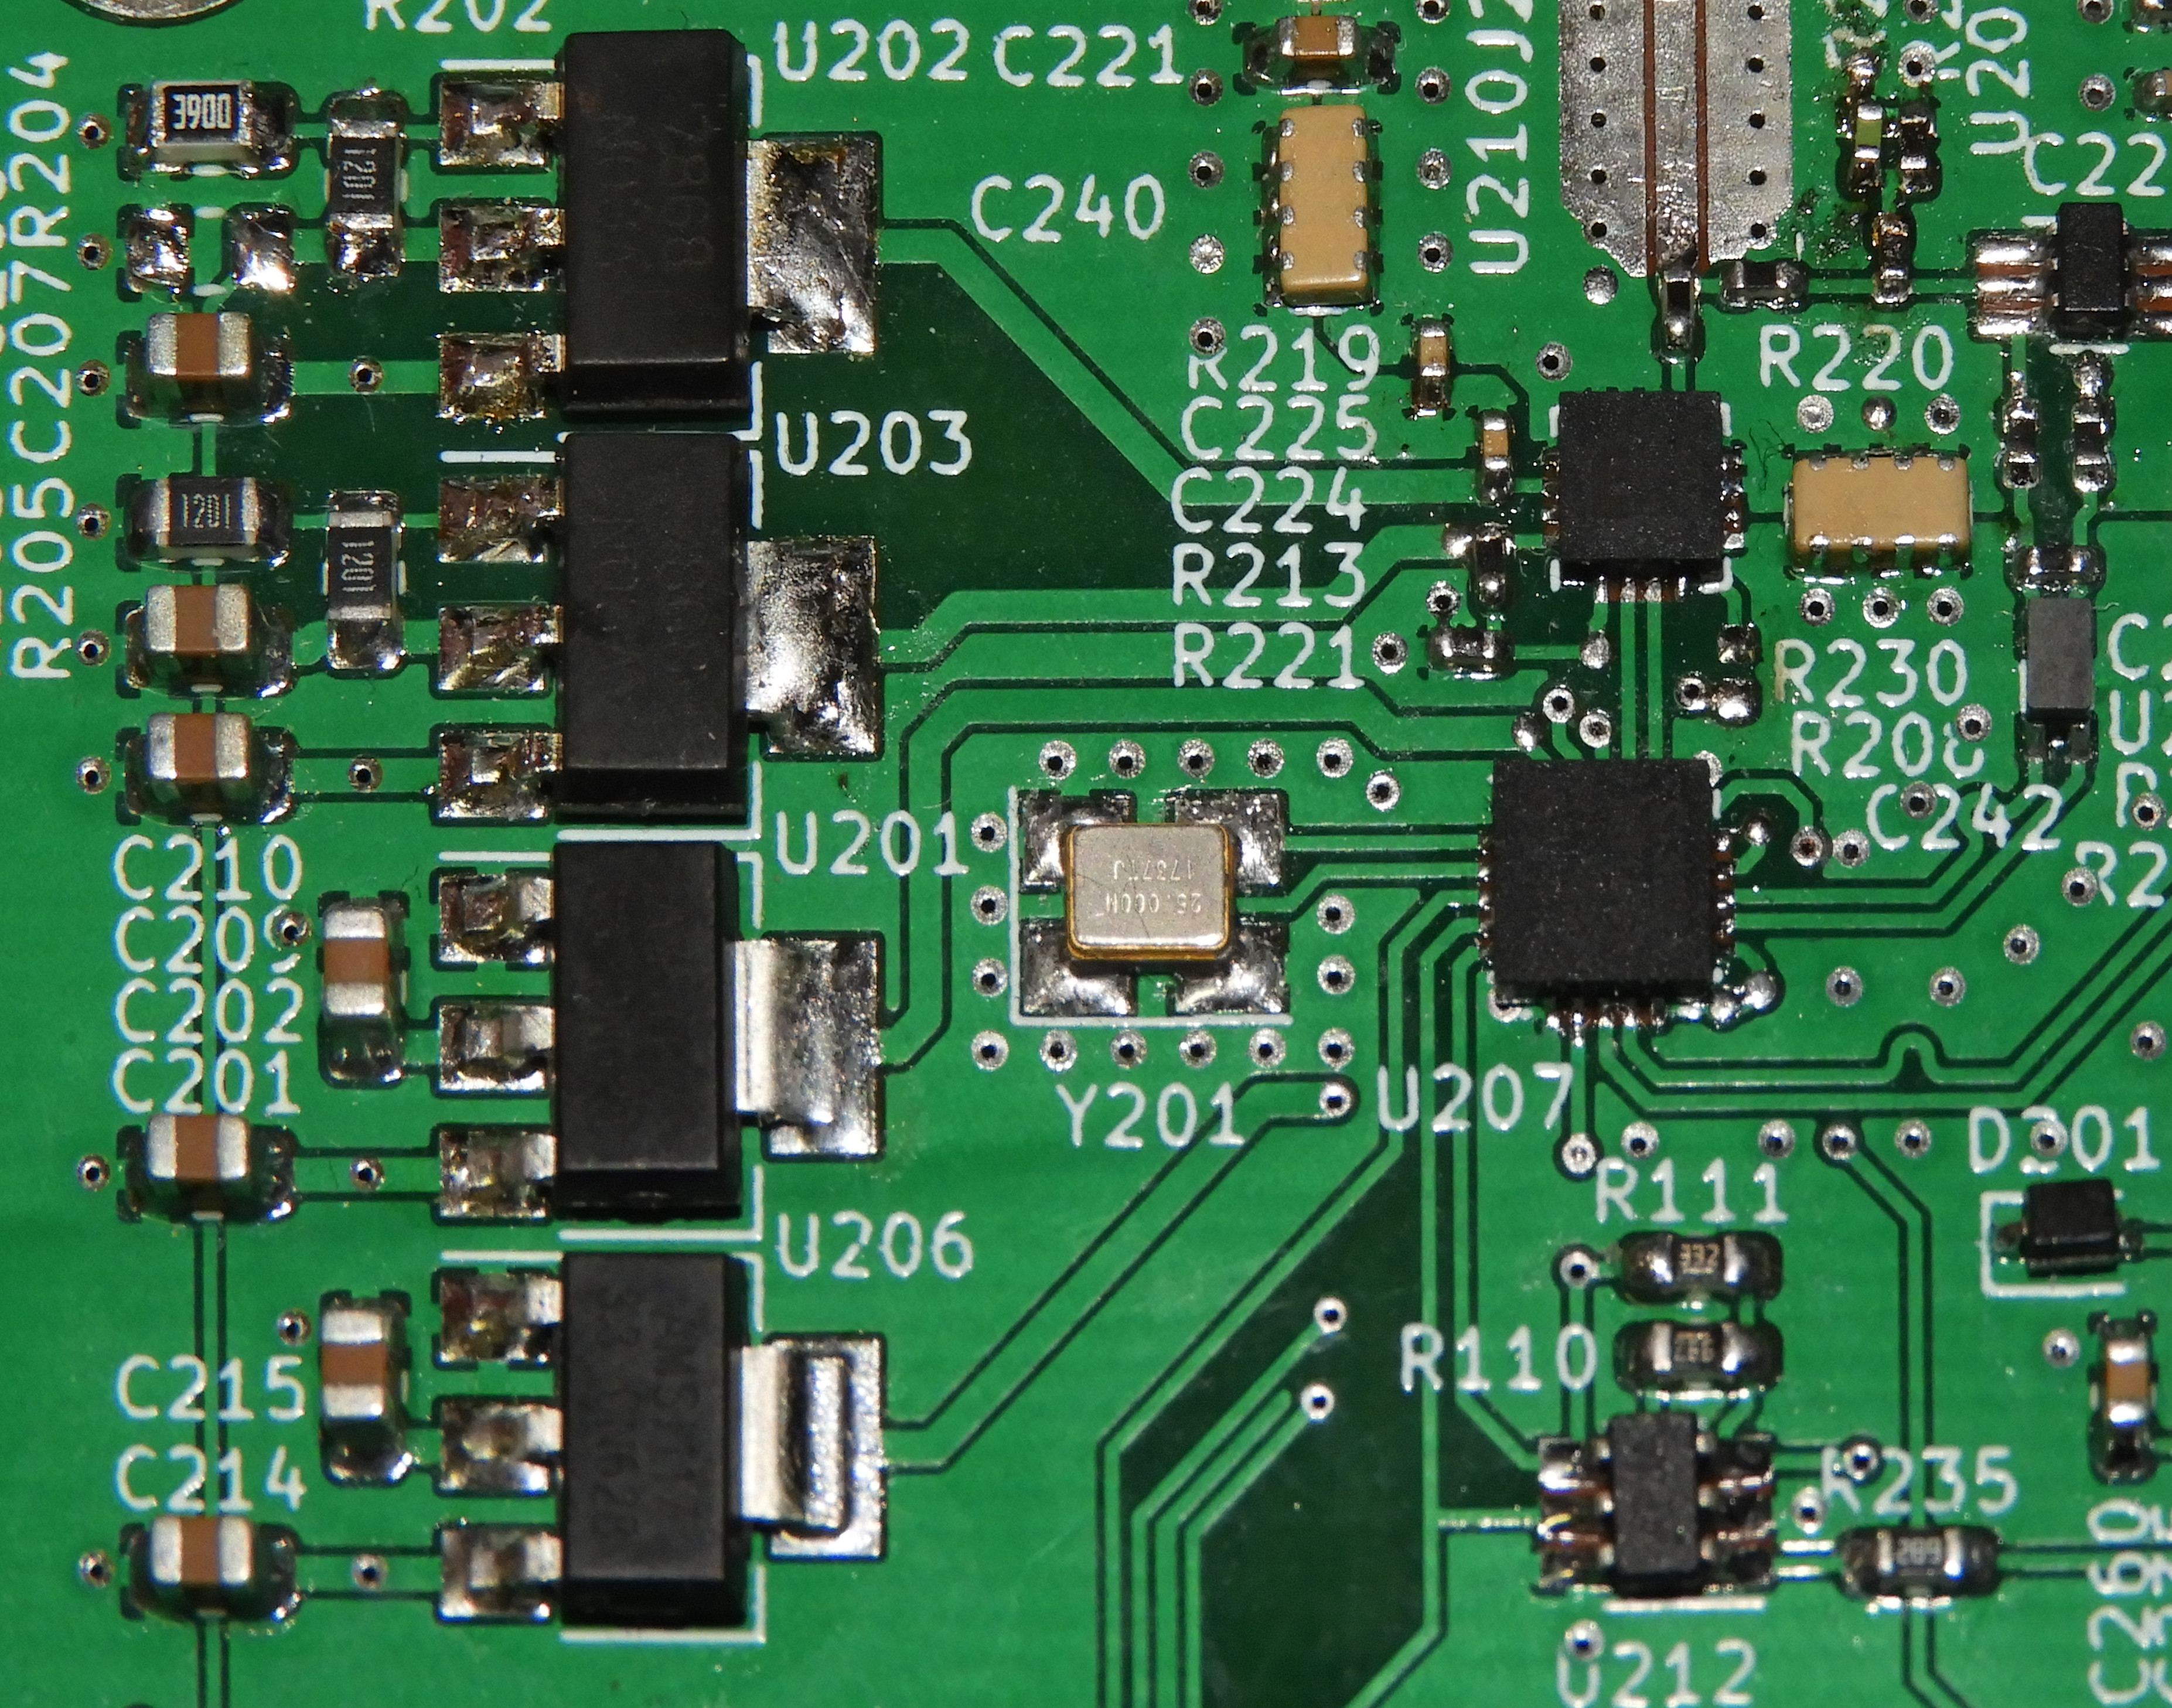
\includegraphics[width=\textwidth,keepaspectratio]{images/pcb/pcb_pll_buffer.jpg}\caption{Fázový závěs, generátor budicích impulzů a napájecí zdroje.}\label{pcb_pll_buffer}
\end{figure}

\begin{figure}[htbp]
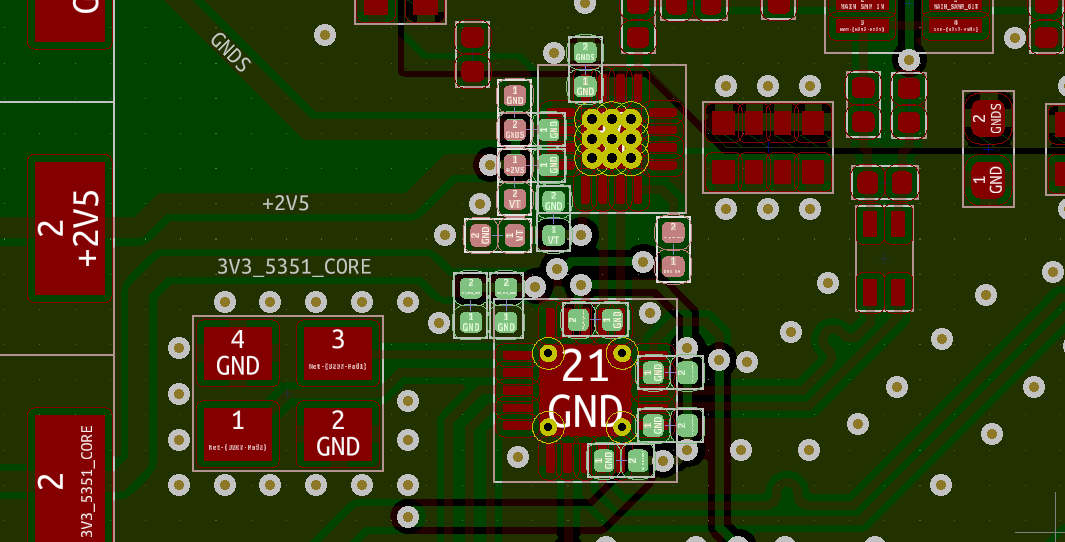
\includegraphics[width=\textwidth,keepaspectratio]{images/pcb/pcb_decoupling.png}\caption{Okolí fázového závěsu a budiče v návrhovém prostředí KiCAD. Červenou barvou je vyznačena vrstva, kde se nachází většina součástek, zeleně vrstva, na které se nachází displej.}\label{pcb_decoupling}
\end{figure}

Na obrázku \ref{pcb_splitter} je okolí testovacího konektoru. Na spodním okraji se nachází budič SY54020, přímo nad ním se nachází rezistivní splitter určený k přizpůsobení budiče a vzorkovače k \SI{50}{\ohm} vedení. Splitter je připojen ke konektoru pomocí koplanárního vedení. Pro zajištění správné impedance a minimálních ztrát je z koplanárního vedení odstraněna nepájivá maska. U zvoleného výrobce bohužel nebyla k dispozici možnost nechat vyrobit desku plošných spojů bez povrchové úpravy. Možnosti povrchové úpravy byly olovnatý \acrshort{HAL}, bezolovnatý HAL a zlacení ENIG. Podle \cite{pcb_surface} a \cite{pcb_surface_simple} je z těchto možností lepší volba HAL, protože vedení s touto povrchovou úpravou má vlivem menší drsnosti povrchu nižší ztráty.
\begin{figure}[htbp]
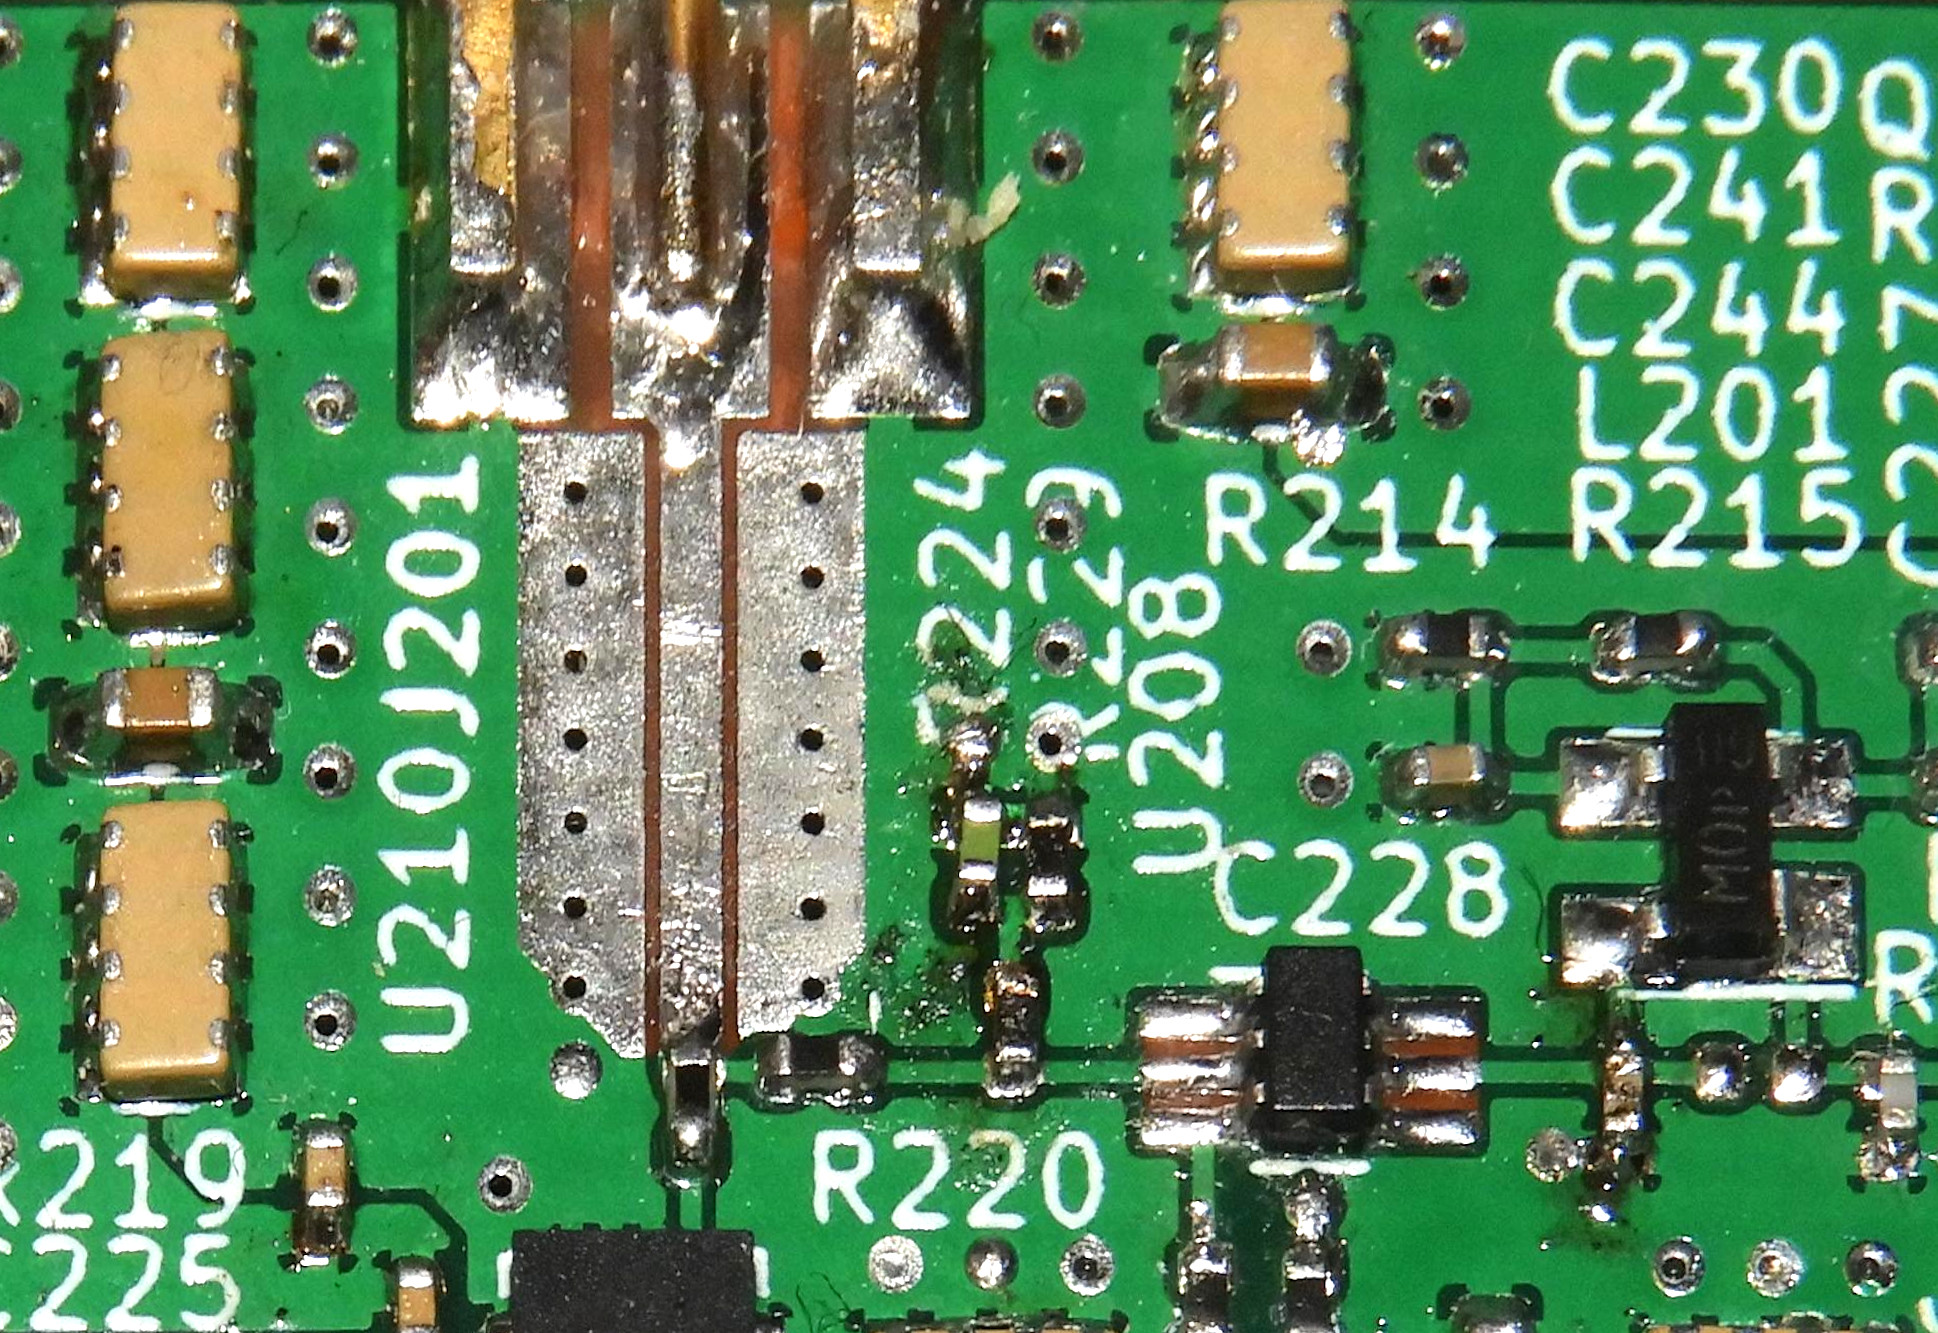
\includegraphics[width=\textwidth,keepaspectratio]{images/pcb/pcb_splitter.jpg}\caption{Budič, rezistivní dělič, koplanární vedení a testovací konektor.}\label{pcb_splitter}
\end{figure}

Na obr. \ref{pcb_main_sampler} je vidět hlavní vzorkovač. V plastovém pouzdře se 6 vývody se nachází diodový můstek SMS3923-081. Pod ním se nachází \SI{150}{\ohm} rezistory a balun, přes které je přivedeno buzení z fázového závěsu Si5351. Tyto komponenty byly použity pro zvýšení souhlasné impedance buzení a tedy zvýšení vstupní impedance vzorkovače. Balun byl později odstraněn, neboť způsoboval rezonanční zákmity na hranách měřeného průběhu. Napravo od vzorkovače je oddělovací zesilovač, lépe je vidět na obr. \ref{pcb_buffer}. Nad tranzistorem BF998 se nachází odpory pro nastavení pracovního bodu. Vpravo se nachází operační zesilovač TL072, ve spodní části odpor, který vede do proudového zdroje, který se využívá pro autokalibraci.
\begin{figure}[htbp]
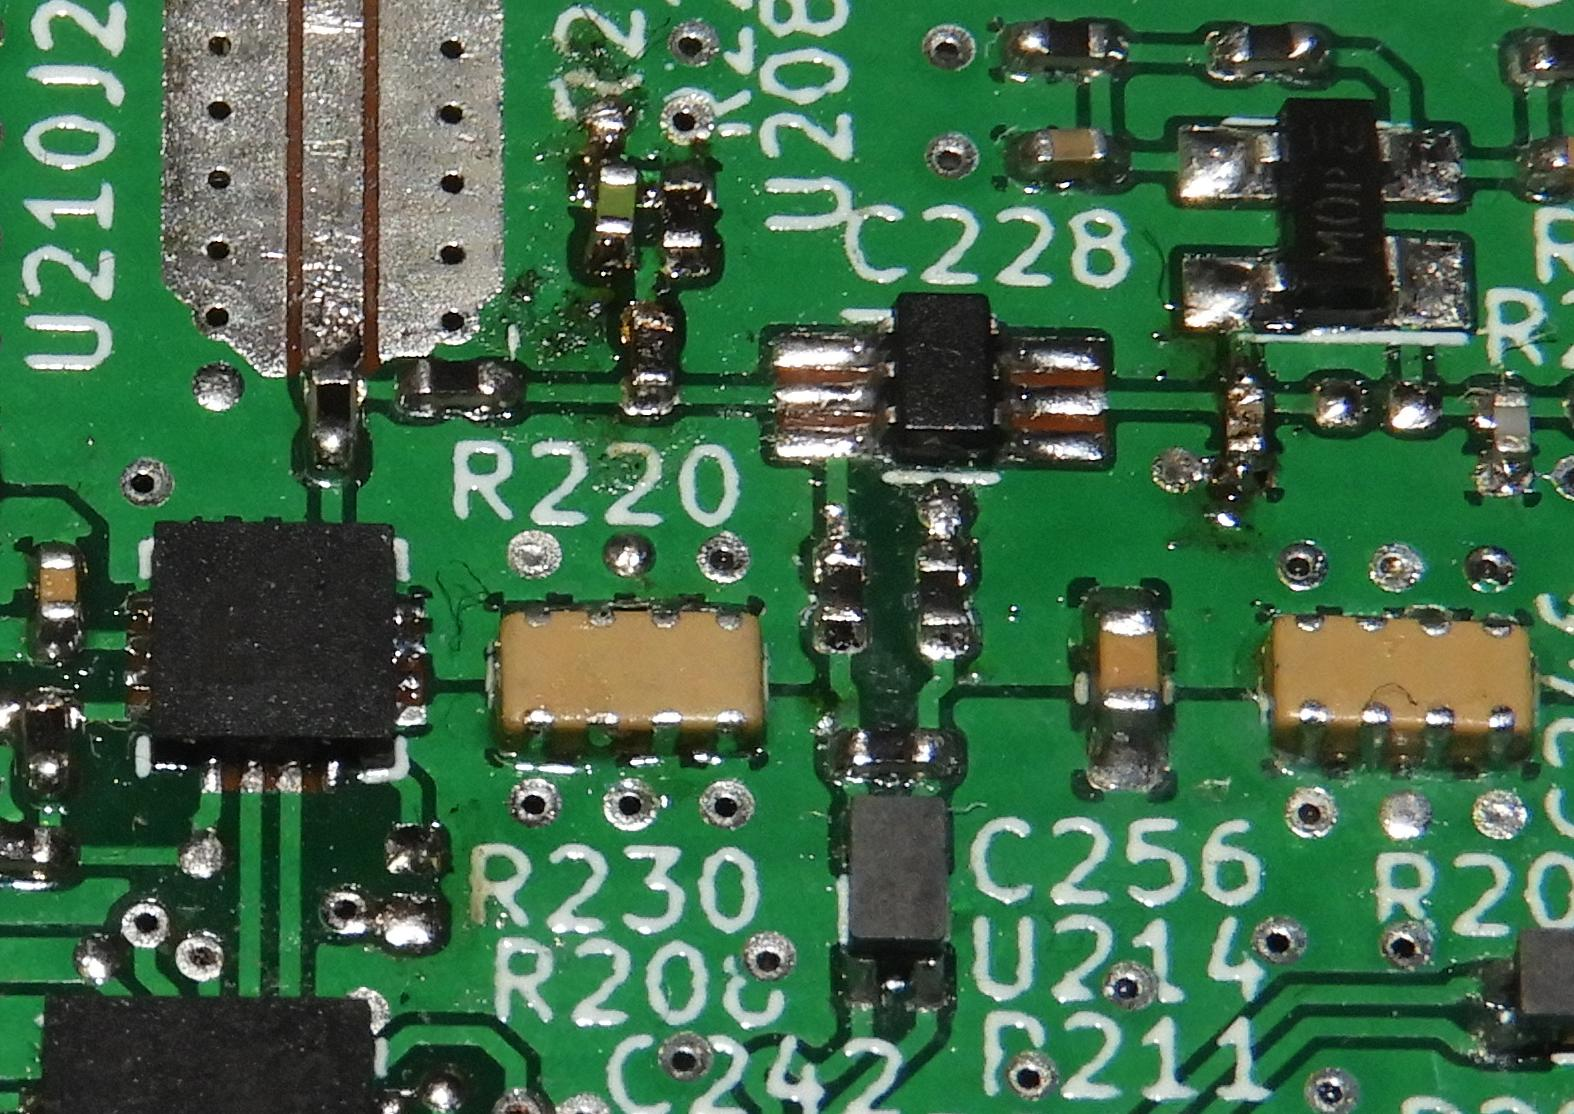
\includegraphics[width=\textwidth,keepaspectratio]{images/pcb/pcb_main_sampler.jpg}\caption{Hlavní vzorkovač.}\label{pcb_main_sampler}
\end{figure}

\begin{figure}[htbp]
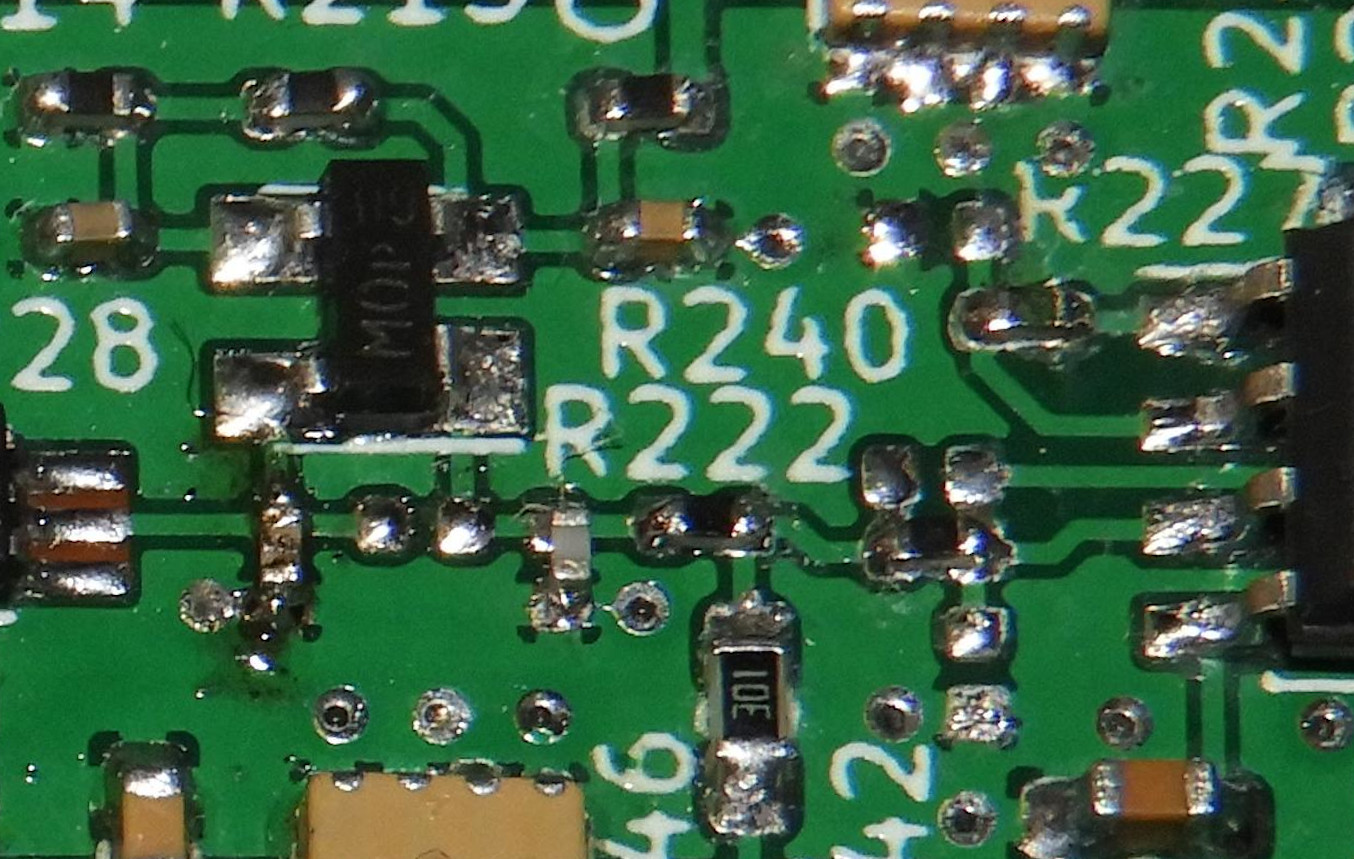
\includegraphics[width=\textwidth,keepaspectratio]{images/pcb/pcb_buffer.jpg}\caption{Oddělovací zesilovač.}\label{pcb_buffer}
\end{figure}

Na obr. \ref{pcb_current_source} je proudový zdroj, který je součástí oddělovacího zesilovače. Pouzdro s 6 vývody v levé části je DAC, kterým se celý zdroj řídí. Ve spodní části se nachází převodník z napětí na proud, vpravo proudové zrcadlo. Tranzistor Q202 je VF tranzistor 2SC5773, jeho kolektor je připojen k oddělovacímu zesilovači.
\begin{figure}[htbp]
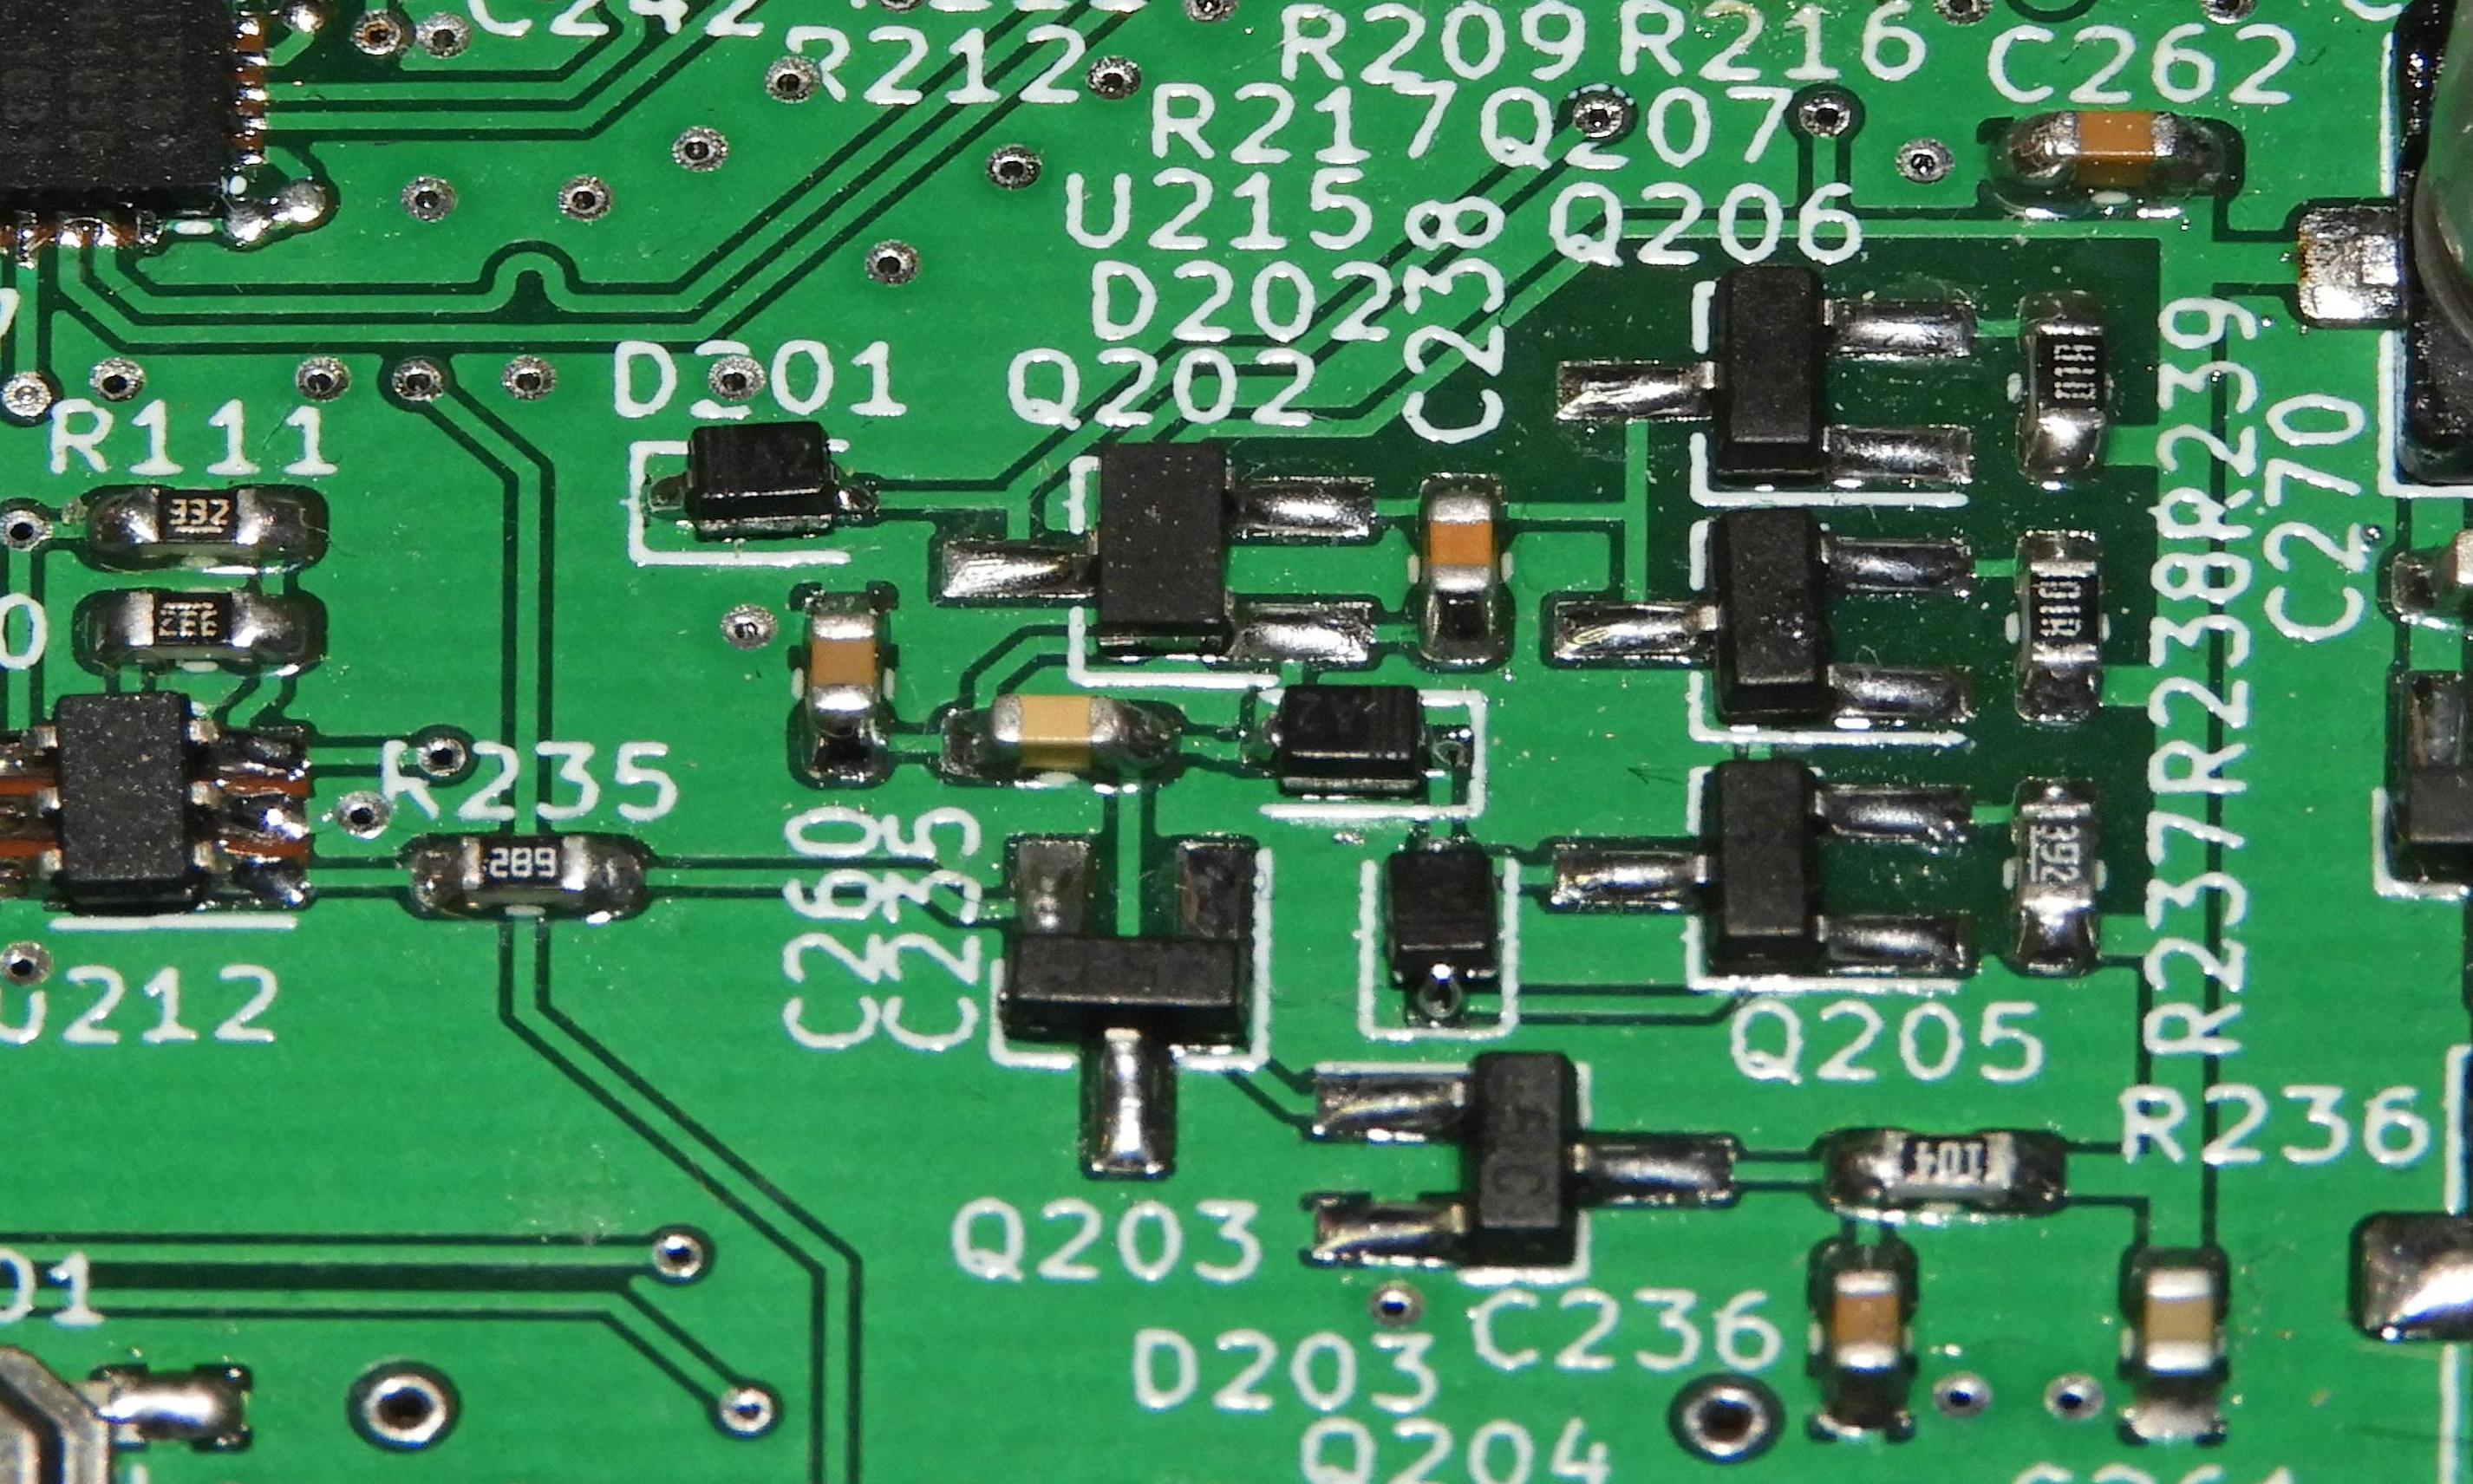
\includegraphics[width=\textwidth,keepaspectratio]{images/pcb/pcb_current_source.jpg}\caption{Proudový zdroj.}\label{pcb_current_source}
\end{figure}

Na obr. \ref{pcb_log} je sekundární vzorkovač a logaritmický detektor. Vzorkovací můstek je opět připojen k fázovému závěsu přes odpory a balun, který byl také později odstraněn. V levé spodní části fotografie je vidět meandr sloužící k vyvážení délek diferenciálního páru. Diferenciální pár, který budí vzorkovací můstek primárního i sekundárního vzorkovače, má takto vyvažované délky vodičů, aby se všechny diody ve vzorkovacích můstcích spínaly ve stejný okamžik. Výstup sekundárního vzorkovače je připojen do operačního zesilovače TL072. Zde se zesílí, aby byl co nejlépe využit rozsah použitého ADC. Zároveň je tento signál přiveden do logaritmického detektoru kvůli možnosti rozšíření dynamického rozsahu měření. Bohužel se později ukázalo, že úroveň šumu v navzorkovaném signálu je příliš vysoká, a tedy detektor nepřináší rozšíření dynamického rozsahu. Dynamický rozsah měření se tedy ve výsledku vylepšuje pomocí průměrování popsaného v rovnici \ref{equation_averaging} podle \cite{HP54100_article_journal}.
\begin{figure}[htbp]
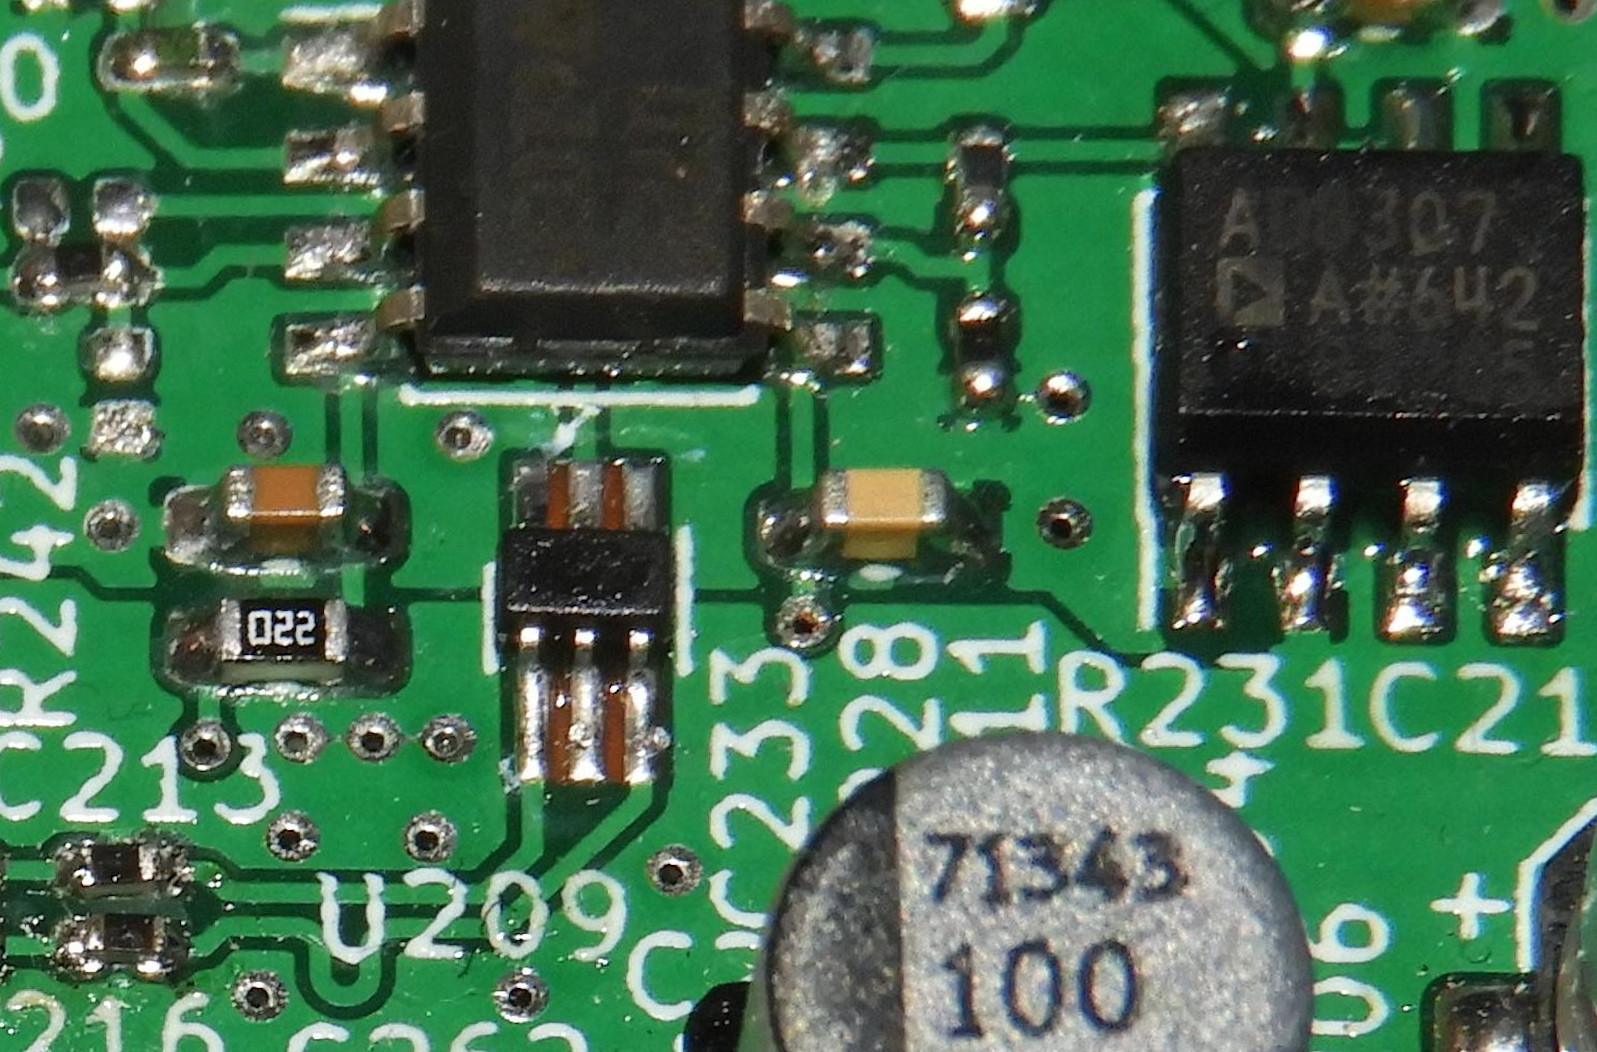
\includegraphics[width=\textwidth,keepaspectratio]{images/pcb/pcb_log.jpg}\caption{Sekundární vzorkovač a logaritmický detektor.}\label{pcb_log}
\end{figure}

Na fotografii \ref{pcb_analog_supply} je symetrický spínaný zdroj pro analogové části reflektometru. Napájí oddělovací zesilovač, proudový zdroj oddělovacího zesilovače a operační zesilovač. V šestinohém pouzdře je samotný měnič MT3608, v těsné blízkosti jsou umístěny blokovací keramické kondenzátory a zpětná vazba kladné napájecí větve. Nalevo od cívky měniče se nachází nábojová pumpa, která vytváří zápornou napájecí větev. Mezi elektrolytickými kondenzátory v levé části se nachází aktivní filtr záporné napájecí větve, jehož zapojení se nachází ve schématu \ref{analog_source_section_schematic}.
\begin{figure}[htbp]
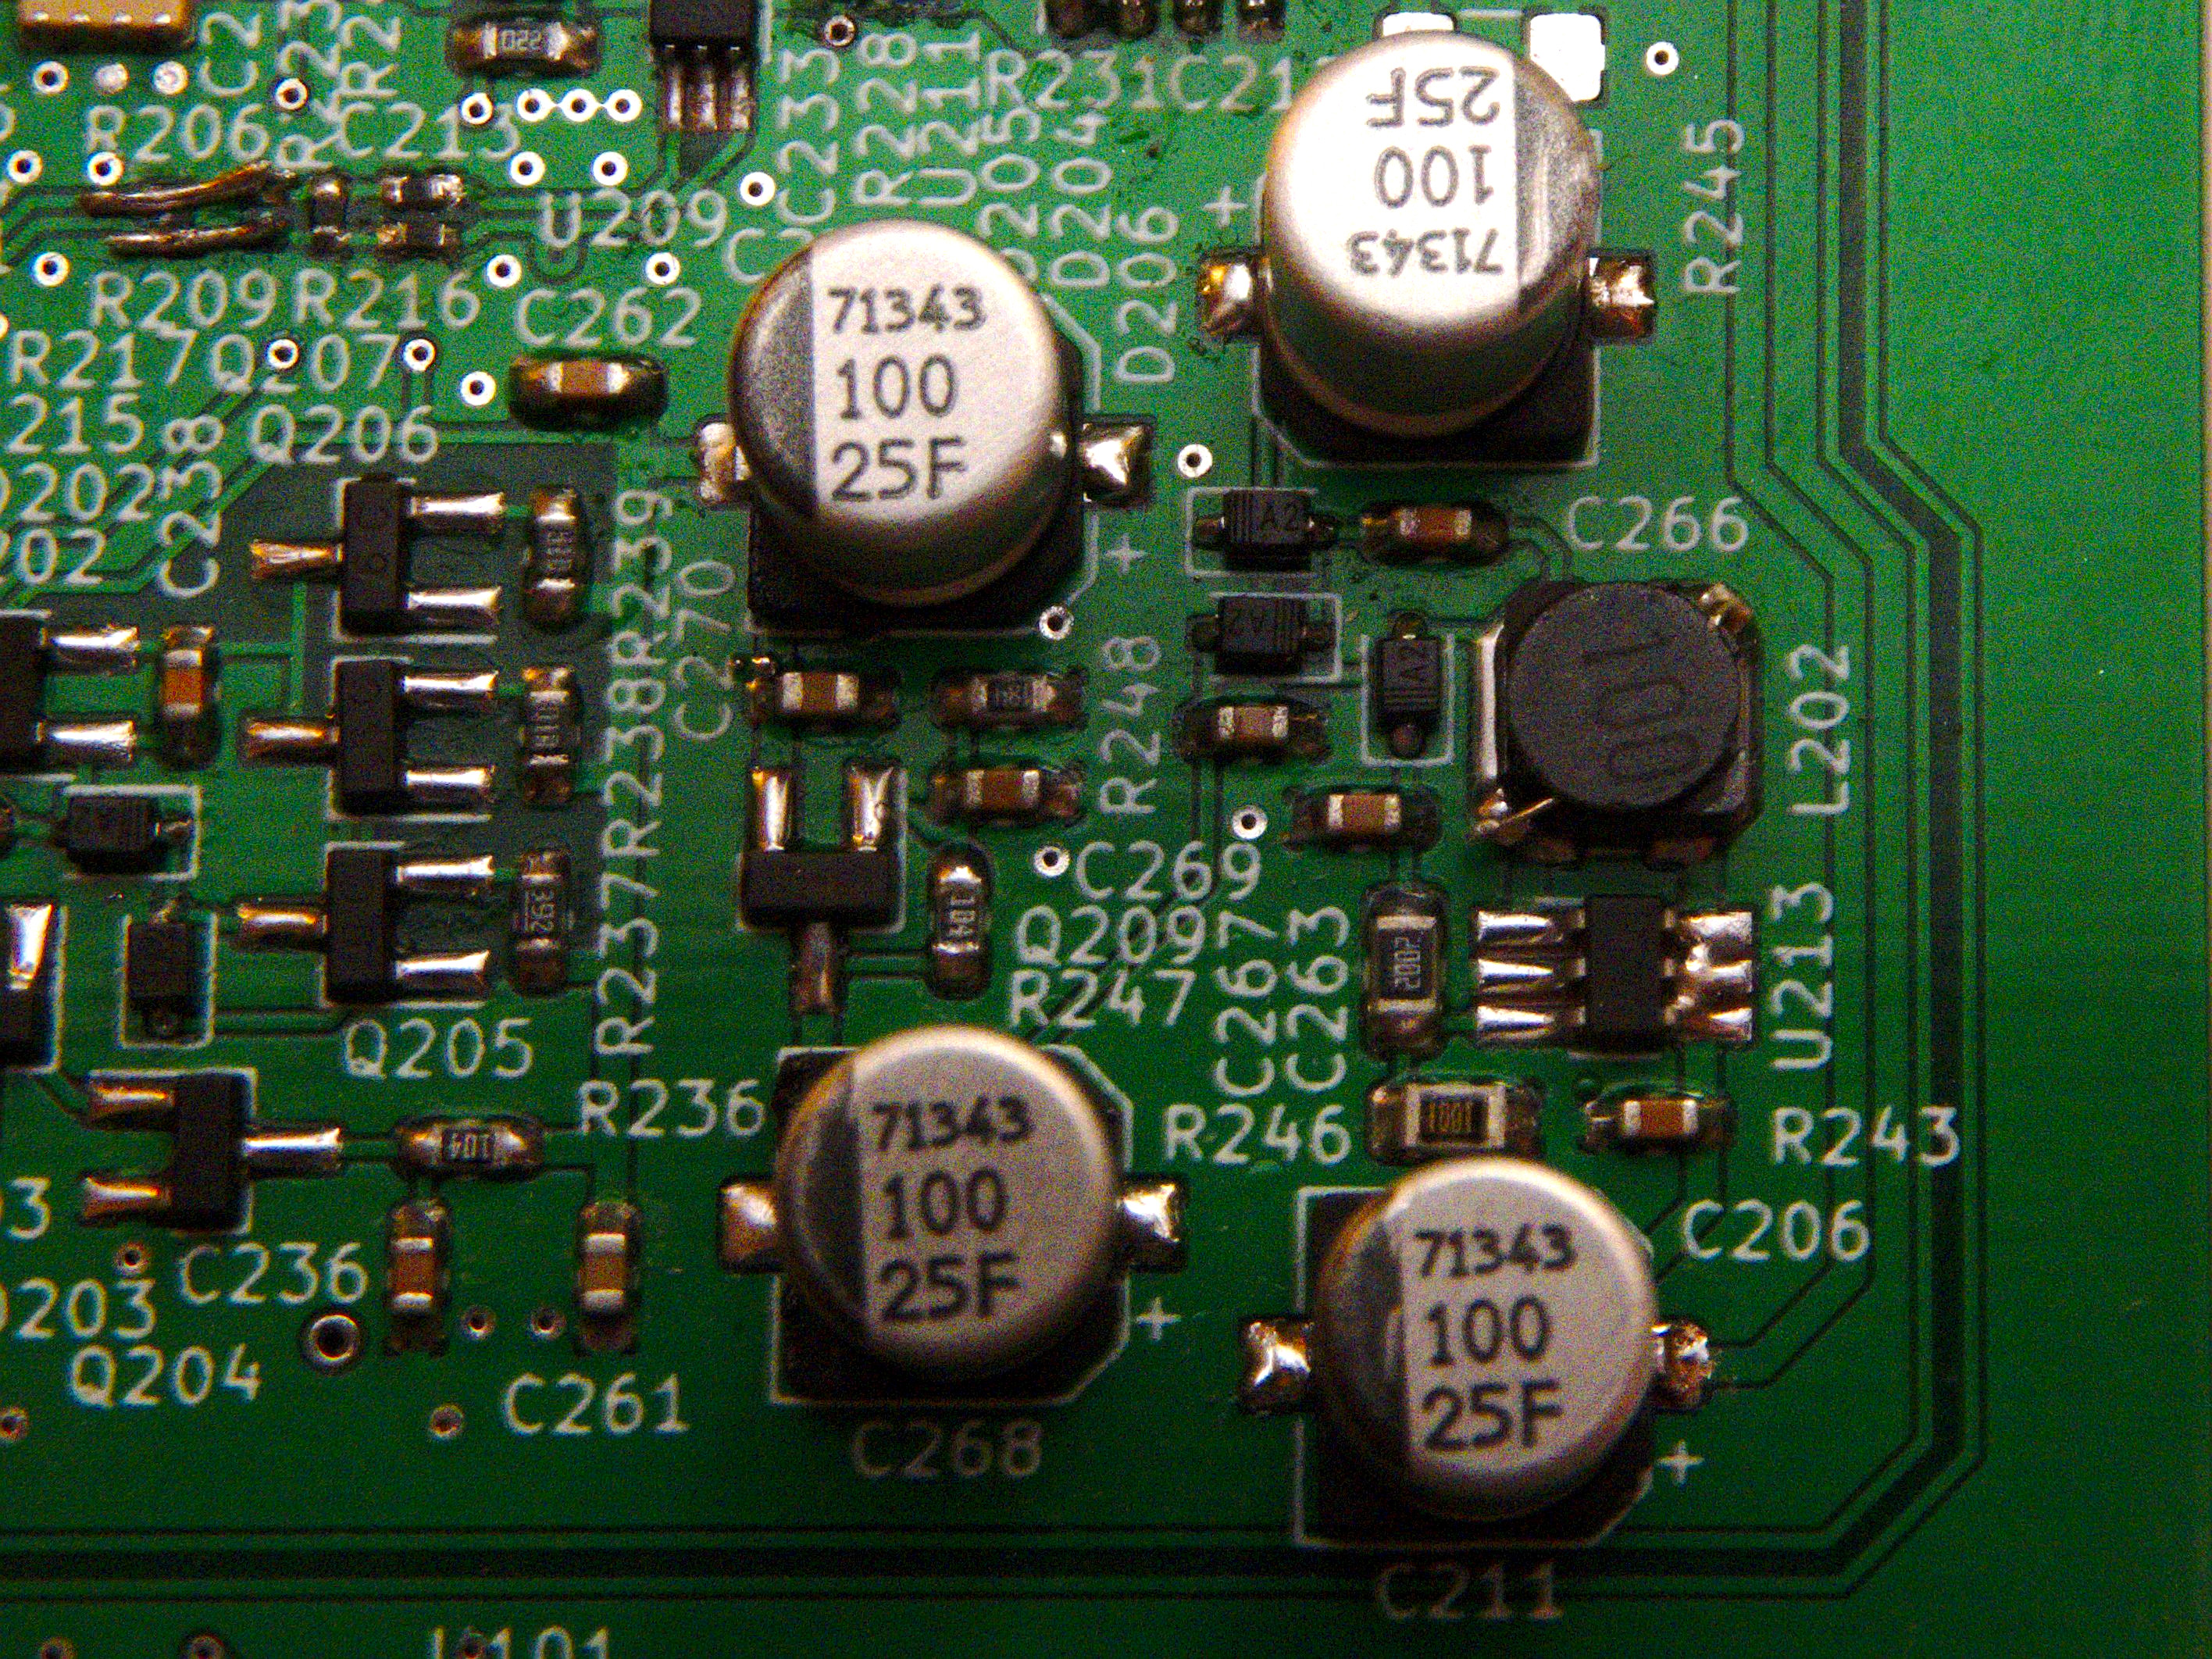
\includegraphics[width=\textwidth,keepaspectratio]{images/pcb/pcb_analog_supply.jpg}\caption{Kombinovaný symetrický zdroj pro analogové části reflektometru.}\label{pcb_analog_supply}
\end{figure}